\documentclass[11pt]{article}

%% Page geometry
\usepackage[a4paper, margin=1in]{geometry}

%% Core math + fonts
\usepackage{amsthm,amsmath,amsfonts,amssymb}
\usepackage{lmodern}
\usepackage{microtype}

%% Citations
\usepackage[authoryear, round]{natbib}

%% Main-article cross-references (assumptions, propositions, equations)
%% are hardcoded just after \begin{document} via \newlabel, so this
%% supplement is self-contained and needs no main.aux / xr-hyper.

%% Colour (for revision marks)
\usepackage{xcolor}

%% Hyperlinks
\usepackage[colorlinks, citecolor=blue, urlcolor=blue, linkcolor=blue]{hyperref}
\usepackage{xurl}

%% Graphics & figures
\usepackage{graphicx}
\graphicspath{{figures/}{./figures/}}
\usepackage{float}
\usepackage{subcaption}
\usepackage{booktabs}
\usepackage{rotating}

%% Float placement. placeins keeps floats inside their section, which is what
%% stops them accumulating into a queue that flushes late -- into the reference
%% list. The LaTeX default fractions are left alone on purpose: overriding
%% textfraction lets a float fill almost a whole page, and on the title page
%% that squeezes the author block.
\usepackage[section]{placeins}

%% Algorithms
\usepackage[linesnumbered, ruled, vlined]{algorithm2e}

%% TikZ for diagrams
\usepackage{tikz}
\usetikzlibrary{shapes,arrows,fit,calc,positioning}
\tikzset{box/.style={draw, diamond, thick, text centered, minimum height=0.5cm, minimum width=1cm}}
\tikzset{line/.style={draw, thick, -latex'}}

%% Misc
\usepackage{comment}
\usepackage{dsfont}
\usepackage{enumitem}
\usepackage{changepage}
\usepackage{bm}

%% Theorem environments
\theoremstyle{plain}
\newtheorem{axiom}{Axiom}
\newtheorem{claim}[axiom]{Claim}
\newtheorem{theorem}{Theorem}[section]
\newtheorem{lemma}[theorem]{Lemma}
\newtheorem{assumption}{Assumption}
\newtheorem{proposition}{Proposition}
\newtheorem{corollary}{Corollary}

\theoremstyle{definition}
\newtheorem{definition}[theorem]{Definition}
\newtheorem*{example}{Example}
\newtheorem*{fact}{Fact}

\theoremstyle{remark}
\newtheorem{case}{Case}
\newtheorem{remark}{Remark}

%% Custom math commands
\newcommand{\E}{\mathbb{E}}
\newcommand{\1}{\mathds{1}}
\newcommand{\p}{\mathbb{P}}
\renewcommand{\H}{\mathcal{H}}
\newcommand{\T}{\mathcal{T}}
\newcommand{\ind}{\perp\!\!\!\perp}
\newcommand{\RCT}{\mathrm{RCT}}
\newcommand{\RWD}{\mathrm{RWD}}
\newcommand{\AF}{\mathrm{AF}}
\newcommand{\expit}{\operatorname{expit}}

%% Supplementary-materials numbering: everything carries an "S" prefix
%% so that, e.g., \ref{sm:proofs} reads as "S1" in the main article.
\renewcommand{\thesection}{S.\arabic{section}}
\renewcommand{\thesubsection}{\thesection.\arabic{subsection}}
\renewcommand{\theequation}{S\arabic{equation}}
\renewcommand{\thefigure}{S\arabic{figure}}
\renewcommand{\thetable}{S\arabic{table}}
\renewcommand{\theproposition}{S\arabic{proposition}}
\renewcommand{\thecorollary}{S\arabic{corollary}}
\renewcommand{\thealgocf}{S\arabic{algocf}}


\title{Bayesian fusion forests for heterogeneous treatment effects on
  survival from randomised and real-world data\\[0.4em]
   Supplementary Materials}



%% Authors and affiliations match the main manuscript file, as required.
%% Affiliations are set as a numbered block rather than through \thanks:
%% Biostatistics does not allow footnotes.
\author{
  Tijn Jacobs$^{1,\ast}$ \quad
  St\'ephanie L.\ van der Pas$^{1}$ \quad
  Wessel N.\ van Wieringen$^{1, 2}$
}

\date{}

\setlength{\parindent}{0pt}
\setlength{\parskip}{0.8em}


\begin{document}

%% --- Numbers of main-article objects, hardcoded for a self-contained SM. ---
%% Update these if the main-text numbering changes.
\makeatletter
\@namedef{r@ass:sutva}{{1}{}{}{}{}}
\@namedef{r@ass:rct-unconf}{{2}{}{}{}{}}
\@namedef{r@ass:positivity-both}{{3}{}{}{}{}}
\@namedef{r@ass:transport}{{4}{}{}{}{}}
\@namedef{r@ass:censoring}{{5}{}{}{}{}}
\@namedef{r@prop:decomp}{{1}{}{}{}{}}
\@namedef{r@prop:ident}{{2}{}{}{}{}}
\@namedef{r@eq:cf}{{2}{}{}{}{}}
\@namedef{r@eq:aft-model}{{5}{}{}{}{}}
\@namedef{r@eq:m0-decomp-prop}{{11}{}{}{}{}}
\@namedef{r@fig:sim-lambda-u}{{1}{}{}{}{}}
\@namedef{r@tab:sim-competitors}{{1}{}{}{}{}}
\@namedef{r@fig:cate}{{4}{}{}{}{}}
\makeatother

\maketitle

\begin{center}
\begin{minipage}{0.9\textwidth}
\setlength{\parskip}{0.4em}
\small
\noindent
$^{1}$Department of Mathematics, Vrije Universiteit Amsterdam \\
$^{2}$Department of Epidemiology and Data Science, Amsterdam University Medical Centre

\noindent
$^{\ast}$Corresponding author: Tijn Jacobs, Department of Mathematics, Vrije
Universiteit Amsterdam, \texttt{t.jacobs@vu.nl}.
\end{minipage}
\end{center}

%% Keep the title page to the title and the affiliations: no float may drift
%% onto it and squeeze the author block.
\FloatBarrier

% !TEX root = ../general/main.tex

\subsection{Proofs}\label{sm:proofs}

\paragraph{Proof of Proposition~\ref{prop:decomp}.}
We evaluate $\E[\log T \mid A, X, S]$ for each value of $(A, S)$.

\emph{Case $A = 0$.}
By the definition of $m_0$, the right-hand side of \eqref{eq:decomp} reduces to $m_0(X, S)$, which matches the left-hand side.

\emph{Case $A = 1$, $S = 1$ (RCT).}
Consistency (Assumption~\ref{ass:sutva}) gives $\log T = \log T(1)$ when $A = 1$, and Assumption~\ref{ass:rct-unconf} gives $T(1) \,\ind\, A \mid X, S = 1$, so:
\begin{equation}
\E[\log T \mid A = 1,\, X,\, S = 1] \;=\; \E[\log T(1) \mid X,\, S = 1].
\end{equation}
We split this conditional expectation as:
\begin{equation}
\E[\log T(1) \mid X,\, S = 1] \;=\; \E[\log T(0) \mid X,\, S = 1] \,+\, \E[\log T(1) - \log T(0) \mid X,\, S = 1].
\end{equation}
The first term equals $m_0(X, 1)$ by Assumption~\ref{ass:rct-unconf}.
The second term equals $\tau(X)$ by Assumption~\ref{ass:transport}.

\emph{Case $A = 1$, $S = 0$ (RWD).}
The definition of $c$ in \eqref{eq:cf} rearranges to:
\begin{equation}
\E[\log T \mid A = 1,\, X,\, S = 0] \;=\; m_0(X, 0) \,+\, \tau(X) \,+\, c(X),
\end{equation}
which matches the right-hand side of \eqref{eq:decomp}. \qed

\paragraph{Proof of Proposition~\ref{prop:ident}.}
Part~(i) follows by taking the difference of the $A = 1, S = 1$ and $A = 0, S = 1$ cases of \eqref{eq:decomp}.
Part~(ii) is immediate from rearranging \eqref{eq:cf}.
Part~(iii) follows because \eqref{eq:decomp} restricted to $S = 0$ identifies only $m_0(X, 0)$ and the composite $\tau(X) + c(X)$. \qed




\newpage
\subsection{Structural interpretation of the confounding function}\label{sm:scm}

\paragraph{Context and goal.}
The main text treats the RWD as potentially confounded without specifying the source of the confounding.
The confounding function $c(x)$ was defined in \eqref{eq:cf} as the residual bias in the RWD treated-versus-control contrast that the causal effect $\tau$ does not explain.
This is an operational definition: it says how to compute $c$ from the observed conditional means, but it says nothing about what real-world mechanisms generate the bias.

The aim of this section is to give $c(x)$ a causal-mechanistic interpretation.
We achieve this by introducing a latent random vector $U \in \mathcal{U}$, called the \emph{unmeasured confounder}, which stands in for any prognostic factor that affects survival but was not recorded in $X$.
Examples include frailty, comorbidities, biomarkers, performance status, genotype, and behavioural risk.
Under a structural model that lets $U$ enter the baseline and the treatment effect, the confounding function decomposes into two interpretable terms: an imbalance in the baseline prognostic function between the RWD treatment arms, and a term capturing effect modification by $U$.

The decomposition has three uses.
First, it makes precise what $c(x)$ measures in causal terms.
Second, it identifies the conditions under which $c(x)$ vanishes.
This in turn motivates the shrinkage prior placed on $c$ in the modelling section.
Third, it provides an entry point for sensitivity analyses that bound the magnitude of $c$ in terms of properties of $U$.

\paragraph{Structural outcome model.}
We posit an outcome equation on the log-time scale:
\begin{equation}
\log T(a) \;=\; f_0(X, U) \,+\, a\,\tau^*(X, U) \,+\, \varepsilon, \qquad \varepsilon \,\ind\, (X, U, A, S).
\label{eq:scm}
\end{equation}
The components have the following meanings.
$X \in \mathcal{X}$ is the vector of observed pre-treatment covariates introduced in the main text.
$U \in \mathcal{U}$ is the latent vector of unmeasured covariates described above; it is unknown to the analyst and never enters the likelihood used for inference.
$f_0(X, U)$ is the baseline log-transformed survival under control, that is, the conditional mean of $\log T(0)$ given $(X, U)$.
$\tau^*(X, U) = \E[\log T(1) - \log T(0) \mid X, U]$ is the treatment effect on the log scale conditional on the full covariate vector $(X, U)$.
$\varepsilon$ is an exogenous mean-zero error, independent of $(X, U, A, S)$; its distribution is left unspecified and follows the same flexible nonparametric form used in the main text.
The CATE on the log scale arises as the conditional mean of $\tau^*$ over $U$ given $X$:
\begin{equation}
\tau(x) \;=\; \E[\tau^*(X, U) \mid X = x].
\label{eq:cate-marginal}
\end{equation}
The model imposes additive separability of the baseline and the treatment effect.
It does not restrict the joint distribution of $(X, U, A)$ in the RWD, so the RWD remains free to be confounded through $U$.

\paragraph{Structural form of $c(x)$.}

\begin{proposition}[Structural form of the confounding function]\label{prop:cf-structural}
Under the structural model \eqref{eq:scm} and Assumptions~\ref{ass:sutva}--\ref{ass:transport}, the confounding function admits the decomposition:
\begin{equation}
c(x) \;=\; \underbrace{\E[f_0(X, U) \mid X = x, A = 1, S = 0] - \E[f_0(X, U) \mid X = x, A = 0, S = 0]}_{\text{prognostic imbalance}} \,+\, \underbrace{\delta_\tau(x)}_{\text{effect modification by }U},
\label{eq:cf-structural}
\end{equation}
where:
\begin{equation}
\delta_\tau(x) \;=\; \E[\tau^*(X, U) \mid X = x, A = 1, S = 0] \,-\, \tau(x).
\label{eq:delta-tau}
\end{equation}
\end{proposition}

\begin{proof}
Consistency (Assumption~\ref{ass:sutva}) gives $\log T = \log T(A)$ for every observation.
We evaluate the two conditional expectations entering the definition \eqref{eq:cf} of the confounding function.
In the RWD treated arm:
\begin{equation}
\E[\log T \mid X = x,\, A = 1,\, S = 0] \;=\; \E\bigl[f_0(X, U) + \tau^*(X, U) + \varepsilon \,\big|\, X = x,\, A = 1,\, S = 0\bigr],
\end{equation}
and in the RWD control arm:
\begin{equation}
\E[\log T \mid X = x,\, A = 0,\, S = 0] \;=\; \E\bigl[f_0(X, U) + \varepsilon \,\big|\, X = x,\, A = 0,\, S = 0\bigr].
\end{equation}
The error term contributes zero in both expressions because $\varepsilon$ has mean zero and is independent of $(X, U, A, S)$.
The difference of the two expectations is
\begin{multline}
\E[\log T \mid X = x,\, A = 1,\, S = 0] \,-\, \E[\log T \mid X = x,\, A = 0,\, S = 0] \\
\;=\; \E\bigl[f_0(X, U) \,\big|\, X = x,\, A = 1,\, S = 0\bigr] \,-\, \E\bigl[f_0(X, U) \,\big|\, X = x,\, A = 0,\, S = 0\bigr] \\
\,+\, \E\bigl[\tau^*(X, U) \,\big|\, X = x,\, A = 1,\, S = 0\bigr].
\end{multline}
We subtract $\tau(x)$ from both sides and apply the definition \eqref{eq:cf} of $c(x)$.
The result is \eqref{eq:cf-structural}, with $\delta_\tau(x)$ as in \eqref{eq:delta-tau}.
\end{proof}

\paragraph{Reduction under no unobserved effect modification.}
The structural form simplifies sharply when the treatment effect does not depend on $U$.

\begin{corollary}[Reduction to prognostic imbalance]\label{cor:no-effect-mod}
If $\tau^*(X, U)$ depends on the covariates only through $X$, i.e.\ $\tau^*(X, U) = \tau(X)$, then $\delta_\tau(x) = 0$ and the confounding function reduces to:
\begin{equation}
c(x) \;=\; \E[f_0(X, U) \mid X = x,\, A = 1,\, S = 0] \,-\, \E[f_0(X, U) \mid X = x,\, A = 0,\, S = 0].
\label{eq:cf-baseline}
\end{equation}
\end{corollary}

\begin{proof}
If $\tau^*(X, U) = \tau(X)$, then $\E[\tau^*(X, U) \mid X = x,\, A = 1,\, S = 0] = \tau(x)$, so $\delta_\tau(x) = 0$.
Substitution into \eqref{eq:cf-structural} yields \eqref{eq:cf-baseline}.
\end{proof}

\paragraph{Interpretation of the two components.}
The two pieces of \eqref{eq:cf-structural} have distinct substantive meanings.

The \emph{prognostic imbalance} term reflects that treated and control observations in the RWD differ in their distribution of $U$ given $X$.
Such an imbalance arises whenever treatment assignment in the RWD depends on unmeasured prognostic factors.
For example, suppose $U$ encodes frailty.
At the same observed covariate value $x$, frailer patients are less likely to be assigned the treatment.
Then $U$ is on average lower in the RWD treated arm than in the RWD control arm at the same $x$, and the conditional expectations of $f_0(X, U)$ differ across arms.
The sign and magnitude of the imbalance depend on the strength of the $U$-$A$ association and on the dependence of $f_0$ on $U$.

The term $\delta_\tau(x)$ captures \emph{effect modification by $U$}.
It is non-zero only when $\tau^*$ itself depends on $U$ and the distribution of $U$ given $X$ in the treated RWD arm differs from that in the population.
For intuition, suppose treatment works better for patients with a certain unmeasured trait.
If the RWD selectively treats patients with that trait, the RWD treated arm exhibits a stronger effect than the population CATE.
This piece is identically zero under Corollary~\ref{cor:no-effect-mod}.

\paragraph{When does the confounding function vanish?}
By Proposition~\ref{prop:cf-structural}, $c(x) = 0$ at $x$ whenever both the prognostic imbalance and $\delta_\tau(x)$ vanish.
A simple sufficient condition is the unmeasured-confounder independence $U \,\ind\, A \mid X, S = 0$: the unmeasured covariate is balanced across RWD treatment arms conditional on $X$.
This is the standard no-unmeasured-confounding assumption in the RWD.
Our framework deliberately avoids assuming it; the role of $c(x)$ is precisely to absorb the bias when this independence fails.

\paragraph{Implications for modelling and sensitivity.}
The structural form has two implications for what follows.
First, $c(x)$ is small when prognostic imbalance is mild and effect modification by $U$ is weak.
The shrinkage prior on $c$ \textbf{[PLACEHOLDER: to be introduced in the modelling section]} is then well-justified.
Second, the magnitude of $c(x)$ admits a sensitivity-analysis interpretation: bounds on how strongly $U$ is associated with $A$ in the RWD and with $f_0$ translate into bounds on $c(x)$.
\textbf{[PLACEHOLDER: brief discussion of relevant sensitivity-analysis frameworks (e.g., Rosenbaum, E-values, Robins--Rotnitzky) and where they fit in the paper.]}

\newpage
\subsection{Structural causal model interpretation of the confounding function (expanded)}\label{sm:scm-full}

\paragraph{Context and goal.}
The previous section interprets $c(x)$ through a structural outcome model.
That model is silent on how the other variables in the problem are generated.
It posits a functional form for $\log T(a)$ but leaves the mechanisms behind $X$, $U$, $S$, and $A$ unspecified.
The main-text assumptions, Assumptions~\ref{ass:sutva}--\ref{ass:transport}, carry the remaining structure as conditional independencies.

We give here a fuller treatment via a structural causal model \citep[SCM;][]{pearl2009causality, peters2017elements}.
An SCM specifies a structural equation for every endogenous variable and a joint distribution over exogenous noises.
The resulting framework is still very broad.
It is also a sub-class of the regression model used for inference in the main text.
The SCM has three advantages over the outcome-model treatment.
First, it makes the data-generating mechanism explicit.
Second, it lets us recover the main-text assumptions from a small set of structural conditions.
Third, it provides a mechanism-level language for sensitivity analyses on $c(x)$.

\paragraph{The structural causal model.}
We posit the following SCM over the random vector $(X, U, S, A, T)$:
\begin{equation}
\begin{aligned}
X &\;=\; f_X(N_X),\\
U &\;=\; f_U(X, N_U),\\
S &\;=\; f_S(X, N_S),\\
A &\;=\; f_A(X, U, S, N_A),\\
T &\;=\; f_T(X, U, A, N_T).
\end{aligned}
\label{eq:fscm}
\end{equation}
The exogenous noises $(N_X, N_U, N_S, N_A, N_T)$ are mutually independent.
The structural functions $f_X, \ldots, f_T$ are otherwise unrestricted.
We model the source $S$ as a function of $X$ alone, so that $N_U$ and $N_S$ are independent.
The latent vector $U$ enters every downstream equation, reflecting that we leave its causal role open.
The potential outcomes are obtained by intervention on $A$:
\begin{equation}
T(a) \;:=\; f_T(X, U, a, N_T), \qquad a \in \{0, 1\}.
\label{eq:fscm-po}
\end{equation}
The observational outcome equals $T(A)$ by construction, which recovers consistency.

We further restrict $f_T$ to admit an additive separation of the baseline and the treatment effect on the log-time scale:
\begin{equation}
\log T(a) \;=\; f_0(X, U) \,+\, a\,\tau^*(X, U) \,+\, \varepsilon,
\label{eq:fscm-outcome}
\end{equation}
where $\varepsilon = \varepsilon(N_T)$ has mean zero and is independent of $(X, U, A, S)$.
Equation~\eqref{eq:fscm-outcome} recovers the outcome model of the previous section.
The remaining equations in \eqref{eq:fscm} are new.
They expose the selection mechanism $f_S$ and the treatment-assignment mechanism $f_A$ that the outcome model left implicit.

\paragraph{Graphical representation.}
The SCM induces the directed acyclic graph in Figure~\ref{fig:scm-dag}.
The graph displays the causal mechanisms and makes the role of $U$ visible.
The arrow $U \to A$ is the source of confounding in the RWD.
The same arrow is degenerate in the RCT under the randomisation restriction below.

\begin{figure}[tb]
\centering
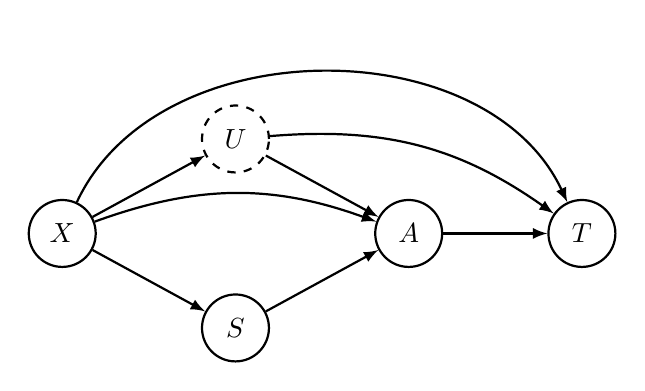
\begin{tikzpicture}[
  >=latex,
  obs/.style={circle, draw, thick, minimum size=0.85cm, inner sep=0pt},
  lat/.style={circle, draw, thick, dashed, minimum size=0.85cm, inner sep=0pt},
  arr/.style={->, thick}
]
  \node[obs] (X) at (0, 0)    {$X$};
  \node[lat] (U) at (2.2, 1.2) {$U$};
  \node[obs] (S) at (2.2, -1.2) {$S$};
  \node[obs] (A) at (4.4, 0)  {$A$};
  \node[obs] (T) at (6.6, 0)  {$T$};

  \draw[arr] (X) -- (U);
  \draw[arr] (X) -- (S);
  \draw[arr] (X) to[bend left=20] (A);
  \draw[arr] (X) to[bend left=65] (T);
  \draw[arr] (U) -- (A);
  \draw[arr] (U) to[bend left=20] (T);
  \draw[arr] (S) -- (A);
  \draw[arr] (A) -- (T);
\end{tikzpicture}
\caption{DAG implied by the SCM \eqref{eq:fscm}. Observed variables are solid; the unmeasured confounder $U$ is dashed. The arrow $U \to A$ is degenerate when $S = 1$ under the RCT randomisation restriction \eqref{eq:fscm-rct}.}
\label{fig:scm-dag}
\end{figure}

\paragraph{Recovering the main-text assumptions.}
Each of the main-text assumptions maps to an explicit constraint on the SCM.
We list them in turn.

\emph{Consistency (Assumption~\ref{ass:sutva})} holds by construction.
The structural equation for $T$ gives $T = f_T(X, U, A, N_T) = T(A)$.

\emph{Unconfoundedness of the RCT (Assumption~\ref{ass:rct-unconf})} restricts $f_A$ on the event $\{S = 1\}$.
The RCT mechanism does not depend on $U$:
\begin{equation}
f_A(X, U, 1, N_A) \;=\; f_A^{\mathrm{RCT}}(X, N_A).
\label{eq:fscm-rct}
\end{equation}
Together with the independence of $N_A$ from $(N_U, N_T)$, this restriction gives $A \,\ind\, (U, T(0), T(1)) \mid X, S = 1$.

\emph{Positivity (Assumption~\ref{ass:positivity-both})} requires that the conditional distribution of $A$ given $(X, S)$ have full support on $\{0, 1\}$ in both sources.
This is a non-degeneracy condition on $f_A$ jointly with the noise $N_A$.

\emph{Cross-source exchangeability (Assumption~\ref{ass:transport})} reduces to two conditions.
First, $f_T$ has no $S$ argument, so the conditional distribution of $T(a)$ given $(X, U)$ does not depend on $S$.
Second, the distribution of $U$ given $X$ is the same in both sources:
\begin{equation}
U \mid X, S = 1 \;\overset{d}{=}\; U \mid X, S = 0.
\label{eq:fscm-uxs}
\end{equation}
The second condition follows from our construction.
We let $S$ depend on $X$ but not on $N_U$, so $U \,\ind\, S \mid X$.
In the selection-diagram language of \citet{bareinboim2016causal}, $S$ acts as a selection node attached to $X$ but disconnected from $U$.

\emph{Conditionally independent censoring (Assumption~\ref{ass:censoring})} is a statement about the censoring mechanism.
It is separate from the outcome SCM and we treat it as outside \eqref{eq:fscm}.

\paragraph{The SCM as a sub-class of the regression model.}
The regression model \eqref{eq:aft-model} places nonparametric priors on the conditional-mean components $m_0$, $\tau$, and $c$.
It is agnostic about the joint distribution of $(X, U, A, S)$.
The SCM \eqref{eq:fscm}--\eqref{eq:fscm-outcome} is one particular family of data-generating processes compatible with that regression model.
Each component of the regression model arises as a conditional expectation under the SCM:
\begin{equation}
m_0(x, s) \;=\; \E[f_0(X, U) \mid X = x, S = s], \qquad \tau(x) \;=\; \E[\tau^*(X, U) \mid X = x],
\label{eq:fscm-induced}
\end{equation}
and $c(x)$ is the residual contrast defined by \eqref{eq:cf}.
The SCM family is still very broad.
It permits arbitrary nonlinear mechanisms, multivariate $U$ of unrestricted dimension, and arbitrary dependence of $A$ on $(X, U)$ in the RWD.
The only structural restrictions are the additive form \eqref{eq:fscm-outcome}, the source-symmetric outcome equation, and the independence \eqref{eq:fscm-uxs} of $U$ from $S$ given $X$.
The first restriction is the AFT modelling choice.
The latter two are precisely what cross-source exchangeability buys us.

\paragraph{Identification within the SCM.}
The identification result of Proposition~\ref{prop:ident} carries over without change.
The RCT slice of the SCM gives $\E[\log T \mid X, A = 1, S = 1] - \E[\log T \mid X, A = 0, S = 1] = \tau(X)$ via \eqref{eq:fscm-rct} and \eqref{eq:fscm-uxs}.
The RWD slice identifies $\tau(x) + c(x)$ as the observed treated-versus-control contrast.
The SCM contributes no additional identifying restrictions.
The latent vector $U$ remains unidentified.

\paragraph{Structural form of $c(x)$.}
We re-derive the structural form of the confounding function within the SCM.
The argument is the same as in Proposition~\ref{prop:cf-structural}.
The SCM makes the conditioning sets transparent.
Decompositions of this form go back to \citet{brumback2004sensitivity} for marginal structural models and \citet{vanderweele2011bias} for general outcomes.

\begin{proposition}[Structural form of $c$ under the SCM]\label{prop:cf-fscm}
Under the SCM \eqref{eq:fscm}--\eqref{eq:fscm-outcome} with restrictions \eqref{eq:fscm-rct} and \eqref{eq:fscm-uxs}, the confounding function satisfies
\begin{equation}
c(x) \;=\; \Delta f_0(x) \,+\, \delta_\tau(x),
\label{eq:cf-fscm}
\end{equation}
with the prognostic-imbalance term
\begin{equation}
\Delta f_0(x) \;=\; \E[f_0(X, U) \mid X = x, A = 1, S = 0] \,-\, \E[f_0(X, U) \mid X = x, A = 0, S = 0],
\label{eq:fscm-delta-f0}
\end{equation}
and the effect-modification term $\delta_\tau(x)$ defined as in \eqref{eq:delta-tau}.
\end{proposition}

\begin{proof}
We use \eqref{eq:fscm-outcome} and the mean-zero independence of $\varepsilon$ to write
\begin{align*}
\E[\log T \mid X{=}x, A{=}1, S{=}0]
  &\;=\; \E[f_0(X, U) + \tau^*(X, U) \mid X{=}x, A{=}1, S{=}0],\\
\E[\log T \mid X{=}x, A{=}0, S{=}0]
  &\;=\; \E[f_0(X, U) \mid X{=}x, A{=}0, S{=}0].
\end{align*}
Subtraction gives the RWD treated-versus-control contrast as a sum of two terms in $f_0$ and one term in $\tau^*$.
We subtract $\tau(x) = \E[\tau^*(X, U) \mid X = x]$ on both sides.
The definition \eqref{eq:cf} of $c(x)$ yields \eqref{eq:cf-fscm}.
\end{proof}

\paragraph{Structural conditions for $c \equiv 0$.}
The SCM lets us read off transparent sufficient conditions under which the confounding function vanishes.

\begin{corollary}[Structural conditions for vanishing $c$]\label{cor:c-zero-fscm}
Under the SCM, $c(x) \equiv 0$ if either of the following holds.
\begin{enumerate}[label=\textup{(\roman*)}]
\item The RWD treatment mechanism does not depend on $U$:
$f_A(X, U, 0, N_A) = f_A^{\mathrm{RWD}}(X, N_A)$.
\item Both $f_0$ and $\tau^*$ depend on covariates only through $X$.
\end{enumerate}
Either condition is sufficient. Neither is necessary.
\end{corollary}

\begin{proof}
Under (i), $U \,\ind\, A \mid X, S = 0$. The conditional distribution of $U$ given $(X, A, S = 0)$ does not depend on $A$. Both $\Delta f_0(x)$ and $\delta_\tau(x)$ vanish.
Under (ii), $f_0(X, U) = f_0(X)$ and $\tau^*(X, U) = \tau(X)$. The conditional expectations in \eqref{eq:cf-fscm} reduce to $f_0(x)$ and $\tau(x)$, so $\Delta f_0 \equiv 0$ and $\delta_\tau \equiv 0$.
\end{proof}

Condition (i) is the standard no-unmeasured-confounding assumption applied to the RWD.
Our framework does not impose it.
The confounding function exists precisely to absorb the bias when (i) fails.
Condition (ii) describes a setting in which $U$ is causally inert for the outcome.
In that case the latent $U$ can be marginalised away without loss.

\paragraph{Parametric instance.}
A linear-Gaussian instance of the SCM makes the structural sources of $c(x)$ tangible.
Take $f_0(X, U) = \beta_0 + \beta_X^\top X + \beta_U U$ and $\tau^*(X, U) = \gamma_0 + \gamma_X^\top X + \gamma_U U$.
Take an RWD treatment mechanism $\p(A = 1 \mid X, U, S = 0) = \Phi(\alpha_0 + \alpha_X^\top X + \alpha_U U)$, with $U \mid X \sim N(0, \sigma_U^2)$.
The two pieces of \eqref{eq:cf-fscm} become
\begin{equation}
\Delta f_0(x) \;=\; \beta_U\,\bigl\{\E[U \mid X{=}x, A{=}1, S{=}0] - \E[U \mid X{=}x, A{=}0, S{=}0]\bigr\},
\end{equation}
and
\begin{equation}
\delta_\tau(x) \;=\; \gamma_U\,\bigl\{\E[U \mid X{=}x, A{=}1, S{=}0] - \E[U \mid X{=}x]\bigr\}.
\end{equation}
Each conditional mean of $U$ in the RWD is a monotone function of $\alpha_U$.
The size of $c(x)$ is governed by three structural quantities.
The first is $\alpha_U$, the strength of confounding in the treatment mechanism.
The second is $\beta_U$, the baseline dependence on $U$.
The third is $\gamma_U$, the strength of effect modification by $U$.
Any one of them being zero kills the corresponding piece.
All three zero recovers $c(x) \equiv 0$.

\paragraph{Sensitivity-analysis framing.}
The SCM provides mechanism-level handles for sensitivity analysis.
Two structural quantities govern the magnitude of $c$.
The first is the dependence of $A$ on $U$ in the RWD, governed by $f_A(\cdot, \cdot, 0, \cdot)$.
The second is the dependence of $f_0$ and $\tau^*$ on $U$.
Standard sensitivity-analysis frameworks parameterise these quantities and induce bounds on the bias.
Rosenbaum bounds \citep{rosenbaum2002observational} constrain the odds-ratio dependence of $A$ on $U$.
The E-value of \citet{vanderweele2017evalue} summarises the joint association strength required to nullify an observed effect.
The framework of \citet{robins2000sensitivity} bounds the bias under prescribed deviations from ignorability.
\citet{YangLiuZengWang2025} apply confounding-function methods to a setting close to ours.
Each framework translates into an implied envelope on $c(x)$ via \eqref{eq:cf-fscm}.
The Bayesian counterpart of these analyses is the shrinkage prior on $c$ introduced in the modelling section.
The prior downweights large values of $c$ without ruling them out.
The data are free to pull $c$ away from zero where the bias is strong.

\paragraph{Implications for modelling.}
The SCM clarifies what the shrinkage prior on $c$ encodes.
Shrinkage towards zero is consistent with the structural picture in which $U$ is approximately balanced across RWD arms at most values of $X$ and effect modification by $U$ is mild.
The prior does not force these conditions.
The shrinkage strength controls how aggressively the RWD informs $\tau$ through the shared baseline $m_0$.
A weaker prior on $c$ trusts the RWD less.
A stronger prior on $c$ approximates the conventional no-unmeasured-confounding assumption in the RWD.
The full SCM treatment makes the prior interpretable as a soft version of Corollary~\ref{cor:c-zero-fscm}(i).
Related RCT--RWD fusion strategies that learn a confounding-bias function from a small experimental sample include \citet{Kallus2018} and \citet{YangLiuZengWang2025}.

\newpage
\subsection{Posterior computation for the HDPM error model}\label{sm:hdp-error}

This section of the Supplementary Materials gives the full hierarchical model after truncation, the conditional distributions of each block of the Gibbs sampler, and recommendations for hyperparameter calibration and practical implementation.

\paragraph{Truncation and full hierarchical model.}
For computation we truncate the top-level stick-breaking at a finite level $K$ \citep{ishwaran2001gibbs}: $u_K = 1$, so $\beta_K = 1 - \sum_{k < K} \beta_k$ and $\beta_k = 0$ for $k > K$.
Conditional on the truncated $\bm{\beta} \in \Delta^{K-1}$ we use the finite-dimensional approximation:
\begin{equation}
\bm{\pi}_s \mid \bm{\beta},\, M_s \;\sim\; \mathrm{Dirichlet}(M_s \beta_1, \ldots, M_s \beta_K),
\label{eq:hdp-pi-prior}
\end{equation}
the standard truncated representation of the hierarchical Dirichlet process \citep{teh2006hierarchical, wang2009variational}.
The approximation becomes exact as $K \to \infty$.
We use a default $K = 50$, which has been adequate in our simulations.
The largest occupied component index should be monitored across iterations to confirm that the truncation does not bind.

We introduce latent cluster assignments $Z_i \in \{1, \ldots, K\}$ such that the latent location for observation $i$ is $\theta_{Z_i}^* - \mu_{S_i}$.
The full hierarchical model is:
\begin{align}
\log T_i \mid Z_i,\, \bm{\theta}^*,\, \bm{\sigma}^2,\, m_0,\, \tau,\, c &\;\sim\; N\!\big(\eta_i,\; \sigma_{S_i}^2\big),\\
\quad\eta_i &\;=\; m_0(X_i, S_i) + A_i\, \tau(X_i) + A_i(1 - S_i)\, c(X_i) + \theta_{Z_i}^* - \mu_{S_i},\\
Z_i \mid \bm{\pi}_{S_i} &\;\sim\; \mathrm{Categorical}(\bm{\pi}_{S_i}),\\
\bm{\pi}_s \mid \bm{\beta},\, M_s &\;\sim\; \mathrm{Dirichlet}(M_s \beta_1, \ldots, M_s \beta_K), \qquad s \in \{0, 1\},\\
\bm{\beta} \mid \gamma &\;\sim\; \mathrm{Stick}_K(\gamma),\\
\theta_k^* &\;\stackrel{\mathrm{iid}}{\sim}\; N(0, \sigma_\theta^2), \qquad k = 1, \ldots, K,\\
m_0, \tau, c &\;\sim\; \mathrm{BART},\\
\sigma_s^2 &\;\sim\; \nu\lambda / \chi^2_\nu, \qquad s \in \{0, 1\},\\
\gamma &\;\sim\; \mathrm{Gamma}(a_\gamma, b_\gamma),\\
M_s &\;\sim\; \mathrm{Gamma}(a_M, b_M), \qquad s \in \{0, 1\},
\end{align}
with $\mu_s = \sum_k \pi_{sk} \theta_k^*$ a deterministic function of $\bm{\pi}_s$ and $\bm{\theta}^*$.
The notation $\mathrm{Stick}_K(\gamma)$ denotes the truncated stick-breaking distribution with $\mathrm{Beta}(1, \gamma)$ breaks.

\paragraph{Gibbs sampler.}
For each observation $i$, define the partial residual:
\begin{equation}
R_i \;:=\; \log T_i - m_0(X_i, S_i) - A_i\, \tau(X_i) - A_i(1 - S_i)\, c(X_i).
\label{eq:app-Ri}
\end{equation}
Conditional on the BART components and the latent cluster assignment $Z_i = k$, we have $R_i \sim N(\theta_k^* - \mu_{S_i}, \sigma_{S_i}^2)$.
One sweep of the sampler executes the following steps.

\paragraph{Step 1 (data augmentation for censoring).}
For each $i$ with $\delta_i = 0$, draw:
\begin{equation}
\log T_i \mid \cdot \;\sim\; \mathrm{TruncatedNormal}(\eta_i,\, \sigma_{S_i}^2;\, [\log C_i, \infty)),
\end{equation}
with $\eta_i$ as defined above.

\paragraph{Step 2 (BART backfitting).}
UPDATE THIS SECTION! We have four forests, also the deviation forest.
The three forests are updated sequentially via Bayesian backfitting \citep{chipman2010bart}.
The working response for each forest is the partial residual obtained by subtracting all other components and the current cluster shift $\theta_{Z_i}^* - \mu_{S_i}$:
\begin{align}
R_i^{(m_0)} &\;=\; \log T_i - A_i \tau(X_i) - A_i(1-S_i) c(X_i) - (\theta_{Z_i}^* - \mu_{S_i}),\\
R_i^{(\tau)} &\;=\; \log T_i - m_0(X_i, S_i) - (1-S_i) c(X_i) - (\theta_{Z_i}^* - \mu_{S_i}), && i \text{ with } A_i = 1,\\
R_i^{(c)} &\;=\; \log T_i - m_0(X_i, 0) - \tau(X_i) - (\theta_{Z_i}^* - \mu_0), && i \text{ with } A_i = 1,\, S_i = 0.
\end{align}
Each working response is treated as Gaussian with mean equal to the relevant forest and per-observation variance $\sigma_{S_i}^2$.
Control observations carry no information about $\tau$.
RCT observations and untreated RWD observations carry no information about $c$.
After the BART updates, recompute $R_i$ from \eqref{eq:app-Ri}.

\paragraph{Step 3 (cluster assignments).}
For each $i$, sample:
\begin{equation}
P(Z_i = k \mid \cdot) \;\propto\; \pi_{S_i, k}\, \phi\!\left(\frac{R_i - (\theta_k^* - \mu_{S_i})}{\sigma_{S_i}}\right), \qquad k = 1, \ldots, K.
\label{eq:app-cluster}
\end{equation}

\paragraph{Step 4 (unconstrained atoms).}
Atoms are sampled in the unconstrained parameterisation and the centring is reapplied deterministically.
Let $n_{sk} = \sum_i \1\{S_i = s, Z_i = k\}$ and $\tilde R_{sk} = \sum_{i : Z_i = k,\, S_i = s} (R_i + \mu_s)$.
The conjugate Gaussian update is precision-weighted across sources:
\begin{equation}
\theta_k^* \mid \cdot \;\sim\; N\!\left(\frac{\sum_{s} \sigma_s^{-2}\, \tilde R_{sk}}{\sigma_\theta^{-2} + \sum_{s} \sigma_s^{-2}\, n_{sk}},\; \bigl(\sigma_\theta^{-2} + \sum_{s} \sigma_s^{-2}\, n_{sk}\bigr)^{-1}\right), \qquad k = 1, \ldots, K.
\label{eq:app-atom-update}
\end{equation}
After updating all atoms, recompute $\mu_s = \sum_k \pi_{sk} \theta_k^*$ and $\theta_{sk} = \theta_k^* - \mu_s$ for $s \in \{0, 1\}$.
As discussed in \citet{yang2010semiparametric}, this parameter-expansion strategy preserves the correct marginal posterior for the centred quantities.

\paragraph{Step 5 (top-level sticks).}
The top-level stick weights are updated using the auxiliary table-count augmentation of \citet{teh2006hierarchical}.
Let $n_{sk} = \sum_i \1\{S_i = s,\, Z_i = k\}$.
For each $(s, k)$ with $n_{sk} > 0$, sample the auxiliary table count $t_{sk}$ via the Antoniak representation \citep{antoniak1974mixtures}:
\begin{equation}
t_{sk} \;=\; \sum_{j=1}^{n_{sk}} B_{sk,j}, \qquad B_{sk,j} \;\sim\; \mathrm{Bernoulli}\!\left(\frac{M_s \beta_k}{M_s \beta_k + j - 1}\right),
\end{equation}
and set $t_{sk} = 0$ if $n_{sk} = 0$.
Let $t_{\cdot k} = t_{0k} + t_{1k}$.
Update the truncated sticks:
\begin{equation}
u_k \mid \cdot \;\sim\; \mathrm{Beta}\!\left(1 + t_{\cdot k},\; \gamma + \sum_{l > k} t_{\cdot l}\right), \qquad k = 1, \ldots, K - 1,
\end{equation}
with $u_K = 1$, and recompute $\beta_k = u_k \prod_{l < k}(1 - u_l)$.

\paragraph{Step 6 (source-specific weights).}
For each $s \in \{0, 1\}$, sample:
\begin{equation}
\bm{\pi}_s \mid \cdot \;\sim\; \mathrm{Dirichlet}(M_s \beta_1 + n_{s1},\, \ldots,\, M_s \beta_K + n_{sK}).
\end{equation}
Recompute $\mu_s$ and the centred atoms.

\paragraph{Step 7 (concentration parameters).}
The concentration parameters $\gamma$ and $M_0, M_1$ are updated using the auxiliary-variable approach of \citet{escobar1995bayesian}.
For $\gamma$, let $K^*$ denote the number of occupied top-level components and $t_{\cdot\cdot} = \sum_{s,k} t_{sk}$ the total table count.
Sample $\eta_\gamma \mid \gamma, t_{\cdot\cdot} \sim \mathrm{Beta}(\gamma + 1, t_{\cdot\cdot})$, then:
\begin{equation}
\gamma \mid \cdot \;\sim\; \omega_\gamma\, \mathrm{Gamma}(a_\gamma + K^*,\, b_\gamma - \log \eta_\gamma) + (1 - \omega_\gamma)\, \mathrm{Gamma}(a_\gamma + K^* - 1,\, b_\gamma - \log \eta_\gamma),
\end{equation}
with $\omega_\gamma / (1 - \omega_\gamma) = (a_\gamma + K^* - 1) / [t_{\cdot\cdot}(b_\gamma - \log \eta_\gamma)]$.
The analogous update for $M_s$ replaces $K^*$ by the source-specific table count $t_{s\cdot} = \sum_k t_{sk}$ and uses $\eta_{M, s} \sim \mathrm{Beta}(M_s + 1, n_s)$.
See \citet[Appendix A]{teh2006hierarchical} for the derivation.

\paragraph{Step 8 (error scale).}
The conjugate update for the residual variance is:
\begin{equation}
\sigma_s^2 \mid \cdot \;\sim\; \mathrm{InverseGamma}\!\left(\frac{\nu + n_s}{2},\; \frac{\nu\lambda + \hat s_s^2}{2}\right), \qquad \hat s_s^2 = \sum_{i : S_i = s} \big(R_i - (\theta_{Z_i}^* - \mu_s)\big)^2, \qquad s \in \{0, 1\}.
\end{equation}

\paragraph{Hyperparameter calibration.}
We adopt the BART defaults of \citet{chipman2010bart} with the AFT-specific adaptations of \citet{henderson2020individualized}: $J = 200$ trees, $\alpha = 0.95$, $\beta = 2$, and the response transformation $y_i^{\mathrm{tr}} = y_i \exp(-\hat\mu_{\mathrm{AFT}})$ based on a preliminary parametric log-normal AFT fit.
The error-scale hyperparameters $\lambda$ and $\sigma_\theta^2$ are calibrated using the Yamato-type approximation \citep{yamato1984characteristic}.
The quantity $\sum_k \pi_{sk}(\theta_k^* - \mu_s)^2 / \sigma_\theta^2$ is approximately $\chi^2_1$ in distribution.
The induced prior on the marginal residual variance $\mathrm{Var}(\varepsilon \mid S = s)$ can therefore be matched in tail probability to a preliminary parametric estimate $\hat\sigma_\varepsilon^2$.
The approximation applies within each source separately.
We use a default tail probability $q = 0.5$.

The concentration hyperpriors are $\gamma \sim \mathrm{Gamma}(a_\gamma, b_\gamma)$ and $M_s \sim \mathrm{Gamma}(a_M, b_M)$ for $s \in \{0, 1\}$, with $a_\gamma = a_M = 2$ and $b_\gamma = b_M = 0.1$.
This places prior mean $20$ on each concentration with prior mode $10$.

\paragraph{Practical considerations.}
Track $\max_i Z_i$ across iterations.
If the largest occupied index equals $K$ in more than a negligible fraction of iterations, the truncation is too tight and $K$ should be increased.
For initialisation, use the standard \citet{chipman2010bart} initialisation for the BART components.
Cluster labels can be assigned by $k$-means on residuals from a preliminary parametric fit.
Set $\bm{\beta} = (1/K, \ldots, 1/K)$, $\bm{\pi}_s = \bm{\beta}$, and $\gamma = M_0 = M_1 = 1$.

\newpage
\subsection{The hierarchical $m_0$ prior as a meta-analytic-predictive prior}\label{sm:map-m0}

The meta-analytic-predictive (MAP) prior of \citet{neuenschwander2010} is a hierarchical Bayesian construction for borrowing strength between studies.
We derive our specification \eqref{eq:m0-decomp-prop} of $m_0(X, S)$ as a function-valued instance of the MAP construction.

\paragraph{Setup of the MAP prior.}
Consider $K$ studies with study-specific parameters $\theta_1, \ldots, \theta_K$.
The MAP prior assumes a Gaussian hierarchical structure:
\begin{align}
\theta_k \mid \mu, \sigma_d^2 &\;\sim\; N(\mu, \sigma_d^2), \qquad k = 1, \ldots, K, \\
\mu &\;\sim\; p(\mu), \\
\sigma_d &\;\sim\; p(\sigma_d).
\label{eq:map-scalar}
\end{align}
The shared mean $\mu$ is the borrowing target.
The heterogeneity variance $\sigma_d^2$ controls how strongly each $\theta_k$ is shrunk towards $\mu$.
Small $\sigma_d$ enforces near-equality of the $\theta_k$, i.e.\ strong borrowing.
Large $\sigma_d$ allows the $\theta_k$ to drift apart, i.e.\ weak borrowing.
The hierarchical structure lets the data determine the degree of borrowing through the posterior of $\sigma_d$.

\paragraph{Function-valued extension.}
Our two studies are the RWD ($s = 0$) and the RCT ($s = 1$), and the study-specific parameter is the prognostic function evaluated at source $s$:
\begin{equation}
\theta_s(X) \;:=\; m_0(X, s), \qquad s \in \{0, 1\}.
\end{equation}
We extend \eqref{eq:map-scalar} from a scalar to a function by replacing the shared mean with a shared function and the Gaussian deviation with a function-valued deviation:
\begin{align}
m_0(X, s) &\;=\; m_0^{\mathrm{sh}}(X) + d_s(X), \qquad s \in \{0, 1\}, \\
m_0^{\mathrm{sh}} &\;\sim\; \mathrm{BART}(\sigma_{h, \mathrm{sh}}^2), \\
d_s &\;\sim\; \mathrm{BART}(\sigma_d^2), \qquad \text{independently across } s.
\label{eq:map-functional}
\end{align}
The BART prior plays the role of a nonparametric prior over functions.
The leaf-prior variance $\sigma_d^2$ now controls cross-source heterogeneity in the same way as the scalar MAP.
The construction is heterogeneous because the deviation is allowed to vary with $X$.
The standard MAP assigns a hyperprior to $\sigma_d$ and lets the data drive borrowing through its posterior.
We instead treat $\sigma_d$ as a calibrated hyperparameter, in line with standard BART practice for leaf-prior scales; the calibration is given below.

\paragraph{Anchored simplification used in the main text.}
The main-text specification \eqref{eq:m0-decomp-prop} anchors at the RCT by setting $d_1 \equiv 0$ and writing $d_0 = d$, giving:
\begin{equation}
m_0(X, S) \;=\; m_0^{\mathrm{sh}}(X) + (1 - S) \cdot d(X).
\end{equation}
This anchors the prognostic function at the RCT level and treats the RWD as the source that drifts from it.
The anchored form is parsimonious and integrates cleanly with the backfitting sampler.
The fully symmetric form \eqref{eq:map-functional} with separate $d_0$ and $d_1$ retains the same identifiability of $\tau$ and $c$ and is preferable when neither source plays the role of a natural reference.

\paragraph{Semiparametric extension of \citet{hupf2021bayesian}.}
The standard MAP \eqref{eq:map-scalar} assumes Gaussian deviations, which is restrictive when one or more studies are outliers.
\citet{hupf2021bayesian} extend MAP to flexible deviations through a Dirichlet-process-based prior on the heterogeneity distribution.
The BART-based deviation in our functional MAP \eqref{eq:map-functional} plays an analogous role at the function level.
It allows the shape of $d_s$ to depart from a parametric form whenever the data demand it, while retaining the borrowing target $m_0^{\mathrm{sh}}$.

\paragraph{Calibration of the borrowing scale.}
We treat $\sigma_d$ as a calibrated hyperparameter rather than sampling it.
The leaf-prior standard deviation of the deviation forest is set by the Chipman--George--McCulloch rule \citep{chipman2010bart}:
\begin{equation}
\sigma_d \;=\; \frac{k_d}{2\sqrt{m_d}},
\label{eq:map-sigma-d}
\end{equation}
where $m_d$ is the number of trees in the deviation forest and $k_d > 0$ is the tuning constant of the Chipman calibration applied to the deviation forest, playing the role of the borrowing-strength dial.
Small $k_d$ shrinks $d$ towards zero and induces strong borrowing of the RWD prognostic towards the RCT prognostic.
Large $k_d$ relaxes the prior and lets $d$ depart further from zero.
We take $k_d = 1$ by default, in line with the uniform Chipman calibration of the main text.
A fully Bayesian alternative is to put a hyperprior on $\sigma_d$ as in the standard MAP \citep{neuenschwander2010}; this trades the simplicity of the BART convention for additional data-driven adaptation of the borrowing strength.

\newpage
\subsection{Outer Gibbs sampler and tree updates}\label{sm:computation}

The posterior is sampled by a blocked Gibbs sampler built on an extended Bayesian backfitting approach \citep{chipman2010bart, hahn2020bayesian}.
One sweep of the sampler is summarised in Algorithm~\ref{alg:outer-gibbs}.
The sampler interleaves data augmentation for censored observations, single-tree reversible-jump updates of the four forests, an update of the borrowing scale $\sigma_d$, and an update of the HDPM error block.

\paragraph{Single-tree reversible-jump updates.}
Each tree-and-step-height pair $(\mathcal{T}_j^f, \mathcal{H}_j^f)$ is updated by one of three reversible-jump proposals: \texttt{GROW}, \texttt{PRUNE}, or \texttt{CHANGE}.
The proposal mechanism follows \citet{chipman2010bart} with the AFT-specific adaptations of \citet{henderson2020individualized}.
Full derivations of the acceptance ratios are given in the references cited above and are not reproduced here.
The conjugate Gaussian update of the leaf step heights is performed jointly with the structural proposal.

\paragraph{Partial residuals.}
Each forest is updated against a partial residual that subtracts the contributions of the other three forests and the current cluster shift $\theta_{Z_i}^* - \mu_{S_i}$ from the residual mixture.
The active subset of observations differs across forests.
The shared baseline $m_0^{\mathrm{sh}}$ uses all observations.
The deviation $d$ uses the RCT observations only.
The treatment effect $\tau$ uses the treated observations from both sources.
The confounding function $c$ uses the treated RWD observations.

\paragraph{Borrowing-scale update.}
The borrowing scale $\sigma_d$ of the heterogeneous MAP prior in Supplementary Materials~\ref{sm:map-m0} is sampled from its conjugate posterior at the end of each sweep.

\paragraph{HDPM error block.}
The blocked update of the error distribution is summarised in Algorithm~\ref{alg:hdp-error}.
Each step corresponds to a conjugate Categorical, Gaussian, Beta, Dirichlet, Gamma, or inverse-Gamma update.
The full mathematical specification of every step is given in Supplementary Materials~\ref{sm:hdp-error}.

\paragraph{Data augmentation for censoring.}
Observations with $\delta_i = 0$ have their unobserved $\log T_i$ drawn from a truncated normal restricted to $[\log C_i, \infty)$ at the start of each sweep \citep{tanner1987}.

\begin{algorithm}[tb]
\caption{Outer Gibbs sampler --- one sweep}
\label{alg:outer-gibbs}
\KwIn{Current forests $(\mathcal{T}_j^f, \mathcal{H}_j^f)$ for $f \in \{m_0^{\mathrm{sh}}, d, \tau, c\}$; observed follow-up times $\tilde T_i$ and event indicators $\delta_i$; HDPM error state; borrowing scale $\sigma_d$.}
\vspace{1ex}

\For{$i = 1$ \KwTo $n$ with $\delta_i = 0$}{
  Draw $\log T_i$ from a truncated normal restricted to $[\log C_i, \infty)$\;
}
\vspace{1ex}

\ForEach{forest $f \in \{m_0^{\mathrm{sh}}, d, \tau, c\}$}{
  \For{$j = 1$ \KwTo $m_f$}{
    Compute the partial residual $\mathcal{R}_j^f$ on the active subset for $f$\;
    Update $(\mathcal{T}_j^f, \mathcal{H}_j^f)$ by a single-tree reversible-jump step\;
  }
}
\vspace{1ex}

Update the borrowing scale $\sigma_d$ from its conjugate posterior\;
\vspace{1ex}

Update the HDPM error block (Algorithm~\ref{alg:hdp-error})\;
\end{algorithm}

\begin{algorithm}[tb]
\caption{HDPM error block --- one update}
\label{alg:hdp-error}
\KwIn{Partial residuals $R_i = \log T_i - m_0^{\mathrm{sh}}(X_i) - S_i d(X_i) - A_i \tau(X_i) - A_i(1 - S_i) c(X_i)$; current atoms $\bm{\theta}^*$, sticks $\bm{\beta}$, source weights $\bm{\pi}_0, \bm{\pi}_1$, concentrations $\gamma, M_0, M_1$, error scales $\sigma_0^2, \sigma_1^2$.}
\vspace{1ex}

\For{$i = 1$ \KwTo $n$}{
  Sample cluster assignment $Z_i$ from the categorical full conditional\;
}
\vspace{1ex}

\For{$k = 1$ \KwTo $K$}{
  Update the unconstrained atom $\theta_k^*$ from its conjugate Gaussian posterior\;
}
Recompute $\mu_s = \sum_k \pi_{sk} \theta_k^*$ and the centred atoms\;
\vspace{1ex}

Sample auxiliary table counts $t_{sk}$ via the Antoniak representation\;
Update top-level sticks $u_k$ from Beta posteriors, then recompute $\beta_k$\;
\vspace{1ex}

\ForEach{$s \in \{0, 1\}$}{
  Update source weights $\bm{\pi}_s$ from a Dirichlet posterior\;
}
Recompute $\mu_s$ and the centred atoms\;
\vspace{1ex}

Update concentrations $\gamma, M_0, M_1$ via the Escobar--West auxiliary-variable scheme\;
\vspace{1ex}

\ForEach{$s \in \{0, 1\}$}{
  Update the error scale $\sigma_s^2$ from its conjugate inverse-gamma posterior\;
}
\end{algorithm}

\newpage
\subsection{Posterior computation \textnormal{\textit{[merged draft for review]}}}\label{sm:posterior-computation-merged}

\textit{Merged and streamlined replacement of the previous Supplementary-Materials sections on the HDPM error model (\ref{sm:hdp-error}) and the outer Gibbs sampler (\ref{sm:computation}). Added as a separate section so the originals can be compared against it before deletion.}

These Supplementary Materials specify the full conditional distribution of every block of the posterior sampler.
We sample the posterior by a blocked Gibbs sampler built on extended Bayesian backfitting \citep{hastie2000bayesian}.
The next subsections describe the outer sampler at a high level and then give the update for each block in turn.

\subsubsection*{Outer Gibbs sampler}

One iteration of the sampler consists of three blocks executed in order: updates of the four forests $f \in \{m_0^{\mathrm{sh}}, d, \tau, c\}$ in turn, an update of the HDPM error block, and data augmentation of the censored event times.
Algorithm~\ref{alg:outer-gibbs-m} summarises one iteration, and Algorithm~\ref{alg:hdp-error-m} summarises the inner update of the HDPM error block.
After burn-in, each iteration produces one posterior sample of the full parameter vector.
The leaf-variance hyperparameters of the four forests, including the borrowing scale $\sigma_d$ of the deviation forest, are treated as calibrated hyperparameters and held fixed across iterations.
Their calibration is described at the end of these Supplementary Materials.

\subsubsection*{Forest updates}

The four forests are updated sequentially by Bayesian backfitting.
Each tree is updated by a birth-death Metropolis-Hastings step on the tree structure, following \citet{chipman2010bart} with the AFT-specific adaptations of \citet{henderson2020individualized}.
The leaf step heights are drawn from their conjugate Gaussian posterior conditional on the tree structure.
Each forest is updated against a partial residual that subtracts the contributions of the other three forests and the current cluster shift $\theta_{Z_i}^* - \mu_{S_i}$ from $\log T_i$.
The active subset of observations differs across forests: $m_0^{\mathrm{sh}}$ uses all observations, $d$ uses the RCT observations, $\tau$ uses the treated observations from both sources, and $c$ uses the treated RWD observations.

\subsubsection*{Updating the HDPM error block}

The HDPM error block updates the latent variables of the nonparametric error distribution: cluster assignments, atoms, top-level stick weights, source-specific weights, concentration parameters, and the per-source residual variances.
All full conditionals are conjugate.
We first state the truncation of the top-level stick-breaking and the resulting hierarchical model, and then give the full conditional for each update in turn.

For computation we truncate the top-level stick-breaking at a finite level $K$ \citep{ishwaran2001gibbs}, setting $u_K = 1$ so that $\beta_K = 1 - \sum_{k < K} \beta_k$ and $\beta_k = 0$ for $k > K$.
Conditional on the truncated $\bm{\beta} \in \Delta^{K-1}$, the source-specific weights have a finite-dimensional Dirichlet prior:
\begin{equation}
\bm{\pi}_s \mid \bm{\beta},\, M_s \;\sim\; \mathrm{Dirichlet}(M_s \beta_1, \ldots, M_s \beta_K),
\label{eq:hdp-pi-prior-m}
\end{equation}
the standard truncated representation of the hierarchical Dirichlet process \citep{teh2006hierarchical, wang2009variational}.
The approximation becomes exact as $K \to \infty$, and we use a default of $K = 50$.
We introduce latent cluster assignments $Z_i \in \{1, \ldots, K\}$ such that the latent location for observation $i$ is $\theta_{Z_i}^* - \mu_{S_i}$, with $\mu_s = \sum_k \pi_{sk} \theta_k^*$.
The full hierarchical model after truncation is then:
\begin{align}
\log T_i \mid \cdot &\;\sim\; N(\eta_i,\; \sigma_{S_i}^2),\\
Z_i \mid \bm{\pi}_{S_i} &\;\sim\; \mathrm{Categorical}(\bm{\pi}_{S_i}),\\
\bm{\pi}_s \mid \bm{\beta},\, M_s &\;\sim\; \mathrm{Dirichlet}(M_s \beta_1, \ldots, M_s \beta_K), \quad s \in \{0, 1\},\\
\bm{\beta} \mid \gamma &\;\sim\; \mathrm{Stick}_K(\gamma),\\
\theta_k^* &\;\stackrel{\mathrm{iid}}{\sim}\; N(0, \sigma_\theta^2), \quad k = 1, \ldots, K,\\
\sigma_s^2 &\;\sim\; \nu\lambda / \chi^2_\nu, \quad s \in \{0, 1\},\\
\gamma &\;\sim\; \mathrm{Gamma}(a_\gamma, b_\gamma),\\
M_s &\;\sim\; \mathrm{Gamma}(a_M, b_M), \quad s \in \{0, 1\},
\end{align}
where $\mathrm{Stick}_K(\gamma)$ denotes the truncated stick-breaking distribution with $\mathrm{Beta}(1, \gamma)$ breaks.

The full conditionals below are all conjugate given the forests and the augmented event times.
We define the partial residual
\begin{equation}
R_i \;:=\; \log T_i - m_0^{\mathrm{sh}}(X_i) - (1 - S_i)\, d(X_i) - A_i\, \tau(X_i) - A_i(1 - S_i)\, c(X_i),
\label{eq:app-Ri-m}
\end{equation}
so that $R_i \mid Z_i = k \sim N(\theta_k^* - \mu_{S_i}, \sigma_{S_i}^2)$.
The cluster assignments are then sampled by
\begin{equation}
P(Z_i = k \mid \cdot) \;\propto\; \pi_{S_i, k}\, \phi\!\left(\frac{R_i - (\theta_k^* - \mu_{S_i})}{\sigma_{S_i}}\right), \quad k = 1, \ldots, K.
\label{eq:app-cluster-m}
\end{equation}

We sample atoms in the unconstrained parameterisation and reapply centring deterministically.
Let $n_{sk} = \sum_i \1\{S_i = s, Z_i = k\}$ and $\tilde R_{sk} = \sum_{i : Z_i = k,\, S_i = s} (R_i + \mu_s)$.
The conjugate Gaussian update is precision-weighted across sources:
\begin{equation}
\theta_k^* \mid \cdot \;\sim\; N\!\left(\frac{\sum_{s} \sigma_s^{-2}\, \tilde R_{sk}}{\sigma_\theta^{-2} + \sum_{s} \sigma_s^{-2}\, n_{sk}},\; \bigl(\sigma_\theta^{-2} + \sum_{s} \sigma_s^{-2}\, n_{sk}\bigr)^{-1}\right), \quad k = 1, \ldots, K.
\label{eq:app-atom-update-m}
\end{equation}
We then recompute $\mu_s = \sum_k \pi_{sk} \theta_k^*$ and the centred atoms $\theta_{sk} = \theta_k^* - \mu_s$.
This parameter-expansion strategy preserves the correct marginal posterior for the centred quantities \citep{yang2010semiparametric}.

The top-level stick weights are updated by the auxiliary table-count augmentation of \citet{teh2006hierarchical}.
For each $(s, k)$ with $n_{sk} > 0$ we sample the auxiliary table count via the Antoniak representation \citep{antoniak1974mixtures}:
\begin{equation}
t_{sk} \;=\; \sum_{j=1}^{n_{sk}} B_{sk,j}, \quad B_{sk,j} \;\sim\; \mathrm{Bernoulli}\!\left(\frac{M_s \beta_k}{M_s \beta_k + j - 1}\right),
\end{equation}
and set $t_{sk} = 0$ when $n_{sk} = 0$.
With $t_{\cdot k} = t_{0k} + t_{1k}$, the truncated sticks are updated by
\begin{equation}
u_k \mid \cdot \;\sim\; \mathrm{Beta}\!\left(1 + t_{\cdot k},\; \gamma + \sum_{l > k} t_{\cdot l}\right), \quad k = 1, \ldots, K - 1,
\end{equation}
with $u_K = 1$ and $\beta_k = u_k \prod_{l < k}(1 - u_l)$.
The source-specific weights then follow
\begin{equation}
\bm{\pi}_s \mid \cdot \;\sim\; \mathrm{Dirichlet}(M_s \beta_1 + n_{s1},\, \ldots,\, M_s \beta_K + n_{sK}), \quad s \in \{0, 1\},
\end{equation}
after which we recompute $\mu_s$ and the centred atoms.

The concentration parameters $\gamma$ and $M_0, M_1$ are updated by the auxiliary-variable scheme of \citet{escobar1995bayesian}.
Let $K^*$ denote the number of occupied top-level components and $t_{\cdot\cdot} = \sum_{s,k} t_{sk}$ the total table count.
We draw $\eta_\gamma \mid \gamma, t_{\cdot\cdot} \sim \mathrm{Beta}(\gamma + 1, t_{\cdot\cdot})$ and then
\begin{equation}
\gamma \mid \cdot \;\sim\; \omega_\gamma\, \mathrm{Gamma}(a_\gamma + K^*,\, b_\gamma - \log \eta_\gamma) + (1 - \omega_\gamma)\, \mathrm{Gamma}(a_\gamma + K^* - 1,\, b_\gamma - \log \eta_\gamma),
\end{equation}
with $\omega_\gamma / (1 - \omega_\gamma) = (a_\gamma + K^* - 1) / [t_{\cdot\cdot}(b_\gamma - \log \eta_\gamma)]$.
The analogous update for $M_s$ replaces $K^*$ by the source-specific table count $t_{s\cdot} = \sum_k t_{sk}$ and uses $\eta_{M, s} \sim \mathrm{Beta}(M_s + 1, n_s)$.
The derivation is in \citet[Appendix A]{teh2006hierarchical}.

The conjugate update of the residual variance closes the block:
\begin{equation}
\sigma_s^2 \mid \cdot \;\sim\; \mathrm{InverseGamma}\!\left(\frac{\nu + n_s}{2},\; \frac{\nu\lambda + \hat s_s^2}{2}\right), \quad \hat s_s^2 = \sum_{i : S_i = s} \big(R_i - (\theta_{Z_i}^* - \mu_s)\big)^2, \quad s \in \{0, 1\}.
\end{equation}

\subsubsection*{Data augmentation for censored event times}

Each iteration closes with data augmentation of the unobserved event times for right-censored observations \citep{tanner1987}.
For every $i$ with $\delta_i = 0$ we draw
\begin{equation}
\log T_i \mid \cdot \;\sim\; \mathrm{TruncatedNormal}\!\left(\eta_i,\, \sigma_{S_i}^2;\, [\log C_i, \infty)\right),
\end{equation}
where $\eta_i = m_0^{\mathrm{sh}}(X_i) + (1 - S_i)\, d(X_i) + A_i\, \tau(X_i) + A_i(1 - S_i)\, c(X_i) + \theta_{Z_i}^* - \mu_{S_i}$ is the conditional mean of $\log T_i$ at the current parameter values.
The augmented values then serve as the working response for the next iteration.

\subsubsection*{Hyperparameter calibration and initialisation}

We adopt the BART defaults of \citet{chipman2010bart} with the AFT-specific adaptations of \citet{henderson2020individualized}: $J = 200$ trees, $\alpha = 0.95$, $\beta = 2$, and the response transformation $y_i^{\mathrm{tr}} = y_i \exp(-\hat\mu_{\mathrm{AFT}})$ based on a preliminary parametric log-normal AFT fit.
The leaf-prior standard deviation of each forest $f$ is calibrated by the Chipman--George--McCulloch rule $\sigma_{h, f} = k_f / (2\sqrt{m_f})$, where $m_f$ is the number of trees in the forest and $k_f > 0$ is a tuning constant.
The borrowing scale of the deviation forest is the special case $\sigma_d = k_d / (2\sqrt{m_d})$.
Small $k_d$ shrinks the deviation $d$ towards zero and induces strong borrowing of the RWD prognostic towards the RCT prognostic; large $k_d$ relaxes the prior and lets $d$ depart further from zero.
The default $k_f = 1$ for every forest $f$ matches the main-text calibration.
The error-scale hyperparameters $\lambda$ and $\sigma_\theta^2$ are calibrated by a Yamato-type approximation \citep{yamato1984characteristic}.
The quantity $\sum_k \pi_{sk}(\theta_k^* - \mu_s)^2 / \sigma_\theta^2$ is approximately $\chi^2_1$, so the induced prior on the marginal residual variance $\mathrm{Var}(\varepsilon \mid S = s)$ can be matched in tail probability to a preliminary parametric estimate $\hat\sigma_\varepsilon^2$.
The approximation is applied within each source separately, with a default tail probability of $q = 0.5$.
For the concentration hyperpriors we use $a_\gamma = a_M = 2$ and $b_\gamma = b_M = 0.1$, which places prior mean $20$ and prior mode $10$ on each concentration.
We initialise the BART components by the defaults of \citet{chipman2010bart}, the cluster labels by $k$-means on residuals from a preliminary parametric fit, and the HDPM weights by $\bm{\beta} = (1/K, \ldots, 1/K)$, $\bm{\pi}_s = \bm{\beta}$, and $\gamma = M_0 = M_1 = 1$.
We track $\max_i Z_i$ across iterations; if it equals $K$ in more than a negligible fraction of iterations, the truncation level $K$ should be increased.

\begin{algorithm}[tb]
\caption{Outer Gibbs sampler, one iteration.}
\label{alg:outer-gibbs-m}
\KwIn{Current forests $(\mathcal{T}_j^f, \mathcal{H}_j^f)$ for $f \in \{m_0^{\mathrm{sh}}, d, \tau, c\}$; current augmented event times $\log T_i$; HDPM error state. Calibrated hyperparameters $\sigma_{h, f}$ for each forest are held fixed.}
\vspace{1ex}

\ForEach{forest $f \in \{m_0^{\mathrm{sh}}, d, \tau, c\}$}{
  \For{$j = 1$ \KwTo $m_f$}{
    Compute the partial residual $\mathcal{R}_j^f$ on the active subset for $f$\;
    Update $\mathcal{T}_j^f$ by a birth-death Metropolis-Hastings step, then draw $\mathcal{H}_j^f$ from its conjugate posterior\;
  }
}
\vspace{1ex}

Update the HDPM error block (Algorithm~\ref{alg:hdp-error-m})\;
\vspace{1ex}

\For{$i = 1$ \KwTo $n$ with $\delta_i = 0$}{
  Draw $\log T_i$ from a truncated normal restricted to $[\log C_i, \infty)$\;
}
\end{algorithm}

\begin{algorithm}[tb]
\caption{Update of the HDPM parameters block.}
\label{alg:hdp-error-m}
\KwIn{Partial residuals $R_i$ from \eqref{eq:app-Ri-m}; current atoms $\bm{\theta}^*$, sticks $\bm{\beta}$, source weights $\bm{\pi}_0, \bm{\pi}_1$, concentrations $\gamma, M_0, M_1$, error scales $\sigma_0^2, \sigma_1^2$.}
\vspace{1ex}

\For{$i = 1$ \KwTo $n$}{
  Sample cluster assignment $Z_i$ from the categorical full conditional in \eqref{eq:app-cluster-m}\;
}
\vspace{1ex}

\For{$k = 1$ \KwTo $K$}{
  Update the unconstrained atom $\theta_k^*$ from its conjugate Gaussian posterior in \eqref{eq:app-atom-update-m}\;
}
Recompute $\mu_s = \sum_k \pi_{sk} \theta_k^*$ and the centred atoms\;
\vspace{1ex}

Sample auxiliary table counts $t_{sk}$ via the Antoniak representation\;
Update top-level sticks $u_k$ from Beta posteriors, then recompute $\beta_k$\;
\vspace{1ex}

\ForEach{$s \in \{0, 1\}$}{
  Update source weights $\bm{\pi}_s$ from a Dirichlet posterior\;
}
Recompute $\mu_s$ and the centred atoms\;
\vspace{1ex}

Update concentrations $\gamma, M_0, M_1$ via the Escobar-West auxiliary-variable scheme\;
\vspace{1ex}

\ForEach{$s \in \{0, 1\}$}{
  Update the error scale $\sigma_s^2$ from its conjugate inverse-gamma posterior\;
}
\end{algorithm}


%% ===== Working notes (status / to-do) — NOT part of the manuscript =====
\begin{comment}
\clearpage
\subsection*{Supplementary Materials: Section structure and writing status}\label{sm:status}

This section records the current state of the methodology section: the proposed final structure, what is drafted, what remains, and the open items that need attention.

\paragraph{Proposed structure of the methodology section.}
\textit{Main text.}
\begin{enumerate}[itemsep=2pt]
  \item \textbf{Causal framework} --- data sources, notation, potential outcomes, censoring formulation, CATE and acceleration factor, assumptions, and the identification trade-off (RWD unconfoundedness against CATE transportability).
  \item \textbf{Accelerated failure time decomposition} --- confounding function $c(x)$, the additive decomposition of $\E[\log T \mid A, X, S]$, identification of $\tau$ and $c$, the AFT outcome model.
  \item \textbf{Nonparametric error distribution} --- hierarchical Dirichlet process mixture of normals (HDPM) with source-specific scales $\sigma_s$.
  \item \textbf{Overview of BART} --- Bayesian additive regression trees as the prior for the regression functions, with the $\mathrm{BART}(m, k, \alpha, \beta)$ shorthand and the tree-structure / step-height prior decomposition.
  \item \textbf{Prior specification} --- BART priors on $m_0^{\mathrm{sh}}, d, \tau, c$ with regularisation matched to each component, the $\sigma_s$ scaled-inverse-$\chi^2$ prior, standardisation of the response, and the hierarchical model summary.
  \item \textbf{Posterior inference} --- hierarchical Bayesian Bootstrap for marginalising the CATE, posterior computation via extended Bayesian backfitting, and ideas for posterior summaries of heterogeneity, borrowing, and residual fit still to be developed.
\end{enumerate}

\textit{Supplementary Materials.}
\begin{enumerate}[label=\Alph*., itemsep=2pt]
  \item \textbf{Proofs} --- Propositions~\ref{prop:decomp} and~\ref{prop:ident}.
  \item \textbf{Structural interpretation of $c$} --- reduced-form structural reading via an unmeasured confounder $U$.
  \item \textbf{Structural causal model for $c$ (expanded)} --- full SCM, DAG, parametric instance, sensitivity-analysis framing.
  \item \textbf{Posterior computation for the HDPM error model} --- truncation, full hierarchical model, eight-step Gibbs sampler with source-specific scales, hyperparameter calibration.
  \item \textbf{Hierarchical $m_0$ as a meta-analytic-predictive prior} --- derivation from the MAP framework of \citet{neuenschwander2010}.
  \item \textbf{Outer Gibbs sampler and tree updates} --- extended Bayesian backfitting algorithm and HDPM error block, with two algorithm boxes.
\end{enumerate}

\paragraph{Status overview.}
\begin{center}
\begin{tabular}{@{}p{4.5cm} l p{8cm}@{}}
\toprule
Section & Status & Notes \\
\midrule
\multicolumn{3}{@{}l}{\emph{Main text.}} \\
1. Causal framework & Drafted & Interval-censoring formulation in place; identification trade-off paragraph proofread. \\
2. AFT decomposition & Drafted & Propositions, proofs, structural-reading remark; meta-comment on the $m_0$ parametrisation still embedded. \\
3. Nonparametric error distribution & Drafted & HDPM construction with per-source $\sigma_s$ and the $\sigma_s^2 \sim \nu\lambda / \chi^2_\nu$ prior calibrated following \citet{chipman2010bart}. \\
4. Overview of BART & Drafted & Concise; tree-structure and step-height prior named explicitly. \\
5. Prior specification & Drafted & Regularisation framing matched to each component; recommended default $k_f = 1$ across the four forests, supported by the prior simulation study. \\
6. Posterior inference & Partially drafted & Hierarchical Bayesian Bootstrap for the ATE drafted; posterior-computation paragraph drafted; itemised placeholders for treatment-effect summaries, heterogeneity, borrowing, and residual fit still to be filled out. \\
\midrule
\multicolumn{3}{@{}l}{\emph{Supplementary Materials.}} \\
A. Proofs & Drafted & Two short proofs. \\
B. Structural interpretation of $c$ & Drafted & Reduced-form reading with proof. \\
C. Structural causal model (expanded) & Drafted & Overlap with B; decide whether to merge or to clearly delineate roles. \\
D. Posterior computation HDPM & Drafted & Eight-step sampler with source-specific scales; atom update is precision-weighted. \\
E. Hierarchical $m_0$ MAP prior & Drafted & Functional MAP derivation; half-Normal scale hyperprior placeholder. \\
F. Outer Gibbs sampler and tree updates & Drafted & Algorithm 1 (outer sweep) and Algorithm 2 (HDPM error block). \\
G. Posterior computation \textit{[merged draft]} & For-review only & Streamlined merger of D and F kept alongside the originals; pending decision before deletion of D + F or of G. \\
\bottomrule
\end{tabular}
\end{center}


\paragraph{Outstanding items.}
\begin{itemize}[itemsep=2pt]
  \item \textbf{Section~6 (Posterior inference) is partially drafted.} The ATE/BB paragraph and the posterior-computation paragraph are in place. The four itemised topics (treatment-effect estimands, heterogeneity, borrowing, residual fit) are still placeholder bullets and need to be expanded into prose.
  \item \textbf{Inline \texttt{[PLACEHOLDER: \ldots]} markers} remain at two locations in the SCM Supplementary Materials: the shrinkage-prior connection in the AFT-decomposition remark, and the sensitivity-analysis framing in the SCM section.
  \item \textbf{``To be verified''} flag inside the conditional-unconfoundedness weakening of randomisation remark (Section~1).
  \item \textbf{Two Supplementary-Materials sections on the structural model} (\texttt{sm:scm} and \texttt{sm:scm-full}). The reduced and expanded versions still overlap.
  \item \textbf{Merged-draft posterior-computation Supplementary-Materials section} (\texttt{sm:posterior-computation-merged}). Streamlined replacement for D and F kept alongside the originals; decide which to keep before circulation.
  \item \textbf{Robust-MAP citation placeholder} (\texttt{[CITE:Schmidli et al.\ 2014]}) in the Supplementary Materials for the heterogeneity hyperprior. Schmidli 2014 is not yet in the bib.
  \item \textbf{General-to-do block} at the foot of the file is the author's working notes. Remove before circulation.
\end{itemize}

\paragraph{Logical next steps.}
\begin{enumerate}[itemsep=2pt]
  \item \textbf{Write out Section~6 (Posterior inference).} Expand the four itemised topics into prose: treatment-effect estimands (CATE, AF, possibly TE-VIM), heterogeneity diagnostics, borrowing diagnostics ($\sigma_d$, $c$-shrinkage), and residual-fit diagnostics (active mixture clusters, $F_0$ vs $F_1$).
  \item \textbf{Resolve the SCM Supplementary-Materials overlap.} Either merge \texttt{sm:scm} and \texttt{sm:scm-full} into one staged section, or sharpen the distinct roles so the reader is not tempted to read both.
  \item \textbf{Resolve the posterior-computation Supplementary-Materials overlap.} Either keep the merged streamlined version (G) and delete D + F, or keep D + F and delete G.
  \item \textbf{Citation to add to the bib.} Schmidli et al.\ 2014 for the robust MAP heterogeneity prior, and replace the corresponding \texttt{[CITE:\ldots]} marker.
  \item \textbf{Final stylistic sweep on Section~6 and the SCM Supplementary Materials.} Sections 1--5 have been audited for \texttt{-ing} openers, em-dashes, prose semicolons, and multi-comma sentences; the remaining material has not.
\end{enumerate}



\hrule

\textbf{GENERAL TO DO}
\begin{itemize}
  \item very thorough check of section Prior specification.
  \item Think about Posterior inference;
  \item check structural causal model section in the Supplementary Materials thoroughly.
  \item Check for other references for the paragrpah on the between-study-heterogeneity of the CATE, and our relaxation of the confoundedness assumption.
\end{itemize}


\hrule




\end{comment}


% % !TEX root = ../general/main.tex
\newpage

% ====================================================================
%  WORKING NOTES. Not part of the final manuscript.
%  One section per planned paragraph, plus a roadmap and parked
%  background material.
% ====================================================================

\section*{Roadmap: structure of the introduction}

\begin{enumerate}
  \item \textbf{Motivation.} Set up the clinical and scientific stakes.
        HTE estimation matters for precision medicine in survival settings.
        RCTs are the gold standard for HTE identification but are typically underpowered for heterogeneity.
        RWD is large and representative of clinical practice but confounded by design.
        Combining the two is attractive in principle.
        Close with: this paper develops a method to do so for survival outcomes.
  \item \textbf{Specific challenges.} What makes the fusion problem hard.
        Three points: (i) unmeasured confounding in the RWD that no design fix can remove; (ii) heterogeneity in the prognostic baseline between RCT and RWD populations even when the causal effect transports; (iii) the survival outcome with right censoring, plus the choice of causal estimand on the time scale.
        Motivate the structural ingredients of the method without revealing them yet.
  \item \textbf{Existing confounding-function approaches.} The frequentist tradition: Yang, Kallus, Yao, Ye, Mao.
  \item \textbf{Bayesian approaches to borrowing and fusion.} A counterpart paragraph on the Bayesian-borrowing literature.
        Cover the commensurate and power-prior MAP tradition (Neuenschwander, Hobbs, Hupf), which targets control-arm augmentation rather than HTE; BART-based external data integration (Zhou \& Ji); and the Causal-ICM multi-task GP framework (Dimitriou et al.).
        Close with the observation that none targets HTE estimation for survival outcomes with explicit confounding-function adjustment.
        That is the gap.
  \item \textbf{Contribution and overview of the method.} What we do and what is new.
        (i) The estimand is the CATE on the log-time scale, equivalently the acceleration factor.
        (ii) Adopt the $m_0 + \tau \cdot A + (1-S)\cdot A \cdot c$ decomposition.
        (iii) Each component receives a BART prior, with hierarchical borrowing on $m_0$ and shrinkage on $c$.
        (iv) The residual is nonparametric via an HDP-CDP that allows source-specific shape.
        (v) Exact posterior inference gives finite-sample uncertainty quantification rather than asymptotic theory.
        Close with the takeaway: efficiency gains over RCT-only HTE estimation when $c$ is small or smoothly varying, with graceful degradation otherwise.
\end{enumerate}

\textbf{Paragraph 6 is removed.} A per-section outline of the paper is redundant.

\textbf{Notes on choices.}
\begin{itemize}
  \item The split between paragraphs 3 and 4 is the main structural decision.
        For a short intro, merge them into one related-work paragraph and lean on the frequentist side.
        For a methods outlet (Biostatistics, JASA Applications \& Case Studies, Bayesian Analysis), keep them separate.
  \item Paragraphs 2 and 5 mirror each other on purpose.
        Paragraph 2 raises three challenges.
        Paragraph 5 resolves them in the same order.
  \item The acceleration-factor justification in paragraph 5 could be its own short paragraph if it needs more space.
        The methodology section already has a careful AF discussion, so keep it inside paragraph 5 unless a reviewer pushes back.
  \item If the paper has a strong applied motivation, drop the example into paragraph 1 to anchor it.
        Otherwise stay generic.
\end{itemize}


\section*{Paragraph 1. Motivation}

\textbf{Draft.}

Heterogeneity in patient response to treatment is central to precision medicine: average effects mask the variation across individuals that drives clinical decisions [Hamburg \& Collins, 2010; Kent et al., 2018].
In survival outcomes --- endpoints that dominate oncology, cardiovascular, and infectious-disease research --- heterogeneous treatment effect (HTE) estimation is particularly consequential, since the benefit of a therapy may depend on baseline disease severity, comorbidities, and other patient-level factors [Henderson et al., 2020].
Randomized controlled trials (RCTs) remain the gold standard for causal effect estimation but are typically powered for marginal effects and underpowered for the subgroup-level contrasts that HTE estimation requires [Rothwell, 2005], and restrictive eligibility further limits the populations to which their conclusions transport.
Real-world data (RWD) from electronic health records, registries, and longitudinal cohorts is increasingly available, larger in scale, and more representative of clinical practice, and is now formally recognized as supplementary evidence by regulators [Sherman et al., 2016; FDA, 2021].
Its cost is unmeasured confounding: without randomization, treatment assignment depends on factors only partially captured by recorded covariates.
The complementary strengths of the two sources motivate a fusion approach that leverages RCT identification with RWD power and representativeness [Colnet et al., 2024].
This paper develops such a method for HTE estimation with survival outcomes, motivated by HIV antiretroviral therapy --- a setting where treatment effect heterogeneity by baseline CD4 count, viral load, and age is well established [Egger et al., 2002] --- and applied to the ACTG175 trial [Hammer et al., 1996] augmented by the Multicenter AIDS Cohort Study (MACS) [Kaslow et al., 1987].

\textbf{To revise.}
\begin{itemize}
  \item Put each sentence on its own line.
  \item Add the BibTeX entries for the bracketed citations and switch them to \texttt{\textbackslash citep}.
  \item Start directly with what we do, then sketch the context.
        Avoid vague openings such as ``\dots is central to precision medicine''.
  \item Check against the writing guidelines.
\end{itemize}



\newpage
\section*{Paragraph 2. Specific challenges}

\textbf{Summary.} Paragraph~2 sets up the three challenges that motivate the methodological choices to come.
\begin{enumerate}
    \item \emph{Unmeasured confounding in the RWD.}
          This breaks the no-unmeasured-confounders assumption.
          Sensitivity analysis addresses it within a single source.
          It does not exploit the identification that an external RCT provides.
    \item \emph{Between-source heterogeneity in the prognostic baseline.}
          The CATE can transport across sources while the control-arm distribution still differs.
          Eligibility, follow-up, calendar time, and case mix all contribute.
    \item \emph{Survival outcome with right censoring.}
          The choice of causal estimand on the time scale matters.
          The hazard ratio is non-collapsible and carries a built-in selection bias.
          The RMST and the acceleration factor are clinically interpretable and causally well behaved.
\end{enumerate}
The paragraph closes by anticipating the contribution.
It addresses all three challenges jointly in a single Bayesian framework.
Paragraph~2 and Paragraph~5 mirror each other on purpose.
Paragraph~2 raises the three challenges, and paragraph~5 resolves them in the same order.

\textbf{Proposed paragraph.}

This fusion problem poses three challenges for survival HTE estimation.
The first is unmeasured confounding in the RWD.
Treatment is not randomized in observational data.
Assignment depends on factors that recorded covariates capture only in part.
The no-unmeasured-confounders assumption is therefore rarely defensible, and the observational contrast is biased for the causal effect \citep{rosenbaum2002observational,vanderweele2017evalue}.
Sensitivity analysis probes robustness within a single study.
It does not use the identification that an external RCT provides.
A fusion approach exploits exactly that identification.
The second challenge is between-source heterogeneity in the prognostic baseline.
The conditional treatment effect may transport across sources while the baseline does not.
RCT and RWD populations differ in eligibility, follow-up, and case mix \citep{stuart2011propensity,degtiar2023review}.
Any of these can shift the control-arm outcome distribution.
A method that pools naively absorbs this shift into biased effect estimates.
The third challenge is the survival outcome itself.
Right censoring leaves the event time unobserved for some subjects.
The causal estimand on the time scale is also a modelling choice.
The hazard ratio is the conventional target, but a poor one for HTE.
It is non-collapsible, and it carries a built-in selection bias under unmeasured heterogeneity \citep{hernan2010,Aalen2015}.
The restricted mean survival time \citep{Royston2013,Uno2014} and the acceleration factor \citep{Brathovde2024} avoid both problems.
Both admit a direct clinical interpretation.
We adopt them as our survival-scale estimands.
We address the three challenges jointly in one Bayesian framework.
The structure of the model mirrors them in turn.

\textbf{Citations.} All nine references already live in \texttt{../general/references.bib}.
The keys:
\begin{itemize}
    \item Rosenbaum (2002): \texttt{rosenbaum2002observational}
    \item VanderWeele \& Ding (2017): \texttt{vanderweele2017evalue}
    \item Stuart et al. (2011): \texttt{stuart2011propensity}
    \item Degtiar \& Rose (2023): \texttt{degtiar2023review}
    \item Hern\'an (2010): \texttt{hernan2010}
    \item Aalen et al. (2015): \texttt{Aalen2015}
    \item Royston \& Parmar (2013): \texttt{Royston2013}
    \item Uno et al. (2014): \texttt{Uno2014}
    \item Brathovde et al. (2024): \texttt{Brathovde2024}
\end{itemize}

\textbf{To adjust.}
\begin{itemize}
  \item Right censoring in general, but interval censoring in particular.
        Observational studies often collect data only at fixed visit times, which gives interval censoring.
        The method should handle that case.
\end{itemize}



\newpage
\section*{Paragraph 3. Confounding-function approaches}

A growing literature combines RCT and observational data to estimate heterogeneous treatment effects by modelling the bias from unmeasured confounding through a \emph{confounding function}.
\citet{YangLiuZengWang2025} introduce this approach in a semiparametric framework for continuous outcomes, deriving the efficiency bounds and jointly estimating the HTE and confounding function via estimating equations.
\citet{Kallus2018} propose an earlier two-step ``experimental grounding'' estimator that learns a parametric bias function from the RCT and uses it to debias an observational HTE estimator.
\citet{Yao2024} extend this strategy to settings where the RWD has incomplete treatment or outcome information, learning the bias function on the overlapping covariate region between the two sources.
In the survival setting, \citet{Ye2025} develop a penalised integrative estimator under an accelerated failure time specification with right censoring and high-dimensional covariates, treating the confounding function as a sparse additive component to be selected jointly with the HTE.
Most closely, \citet{mao2025statistical} target the difference in conditional restricted mean survival times and introduce an \emph{omnibus bias function} that aggregates confounding, censoring, and outcome heterogeneity into a single penalised-sieve nuisance, providing the most direct frequentist counterpart to the framework developed here.
Our contribution departs from these by adopting a Bayesian nonparametric specification throughout: each component of the outcome decomposition receives a BART prior, the residual distribution is modelled with a hierarchical Dirichlet process mixture allowing source-specific shape, and inference proceeds through exact posterior sampling rather than asymptotic semiparametric theory.

\textbf{To do.}
\begin{itemize}
  \item Look in these papers to see what they cite.
  \item Open question: methods for combining data with extended follow-up?
\end{itemize}



\newpage
\section*{Paragraph 4. Bayesian borrowing and fusion}

\textbf{Proposed structure} (single paragraph, two internal halves and a closer).
\begin{itemize}
  \item The traditional Bayesian-borrowing lineage (power priors, MAP, commensurate priors, semiparametric extensions) all target marginal effects or control-arm augmentation, not HTE.
        Close this half with Alt et al. as the survival extension of the lineage.
  \item The newer HTE-focused Bayesian fusion strand: Zhou \& Ji (BART) and Dimitriou et al. (multi-task GP / Causal-ICM).
        Highlight what each does differently (functional vs.\ global bias treatment, GP vs.\ tree-based).
  \item Closing observation: none targets HTE for survival with explicit confounding-function adjustment.
        That is the gap.
\end{itemize}

\textbf{Option A (concise, single paragraph).}

A parallel line of work develops Bayesian methods that borrow information across studies to augment clinical trial analyses.
The foundational contributions target average treatment effects or control-arm augmentation rather than heterogeneous effects: power priors \citep{ibrahim2000power} and the meta-analytic-predictive (MAP) prior of \citet{neuenschwander2010} let external or historical data contribute to the current analysis through a weighted or hierarchical likelihood; commensurate priors \citep{hobbs2011,hobbs2012commensurate} make the borrowing adaptive by shrinking cross-source disagreement to zero when the data are commensurate; and semiparametric extensions \citep{hupf2021bayesian} relax the Gaussian-deviation assumption of the standard MAP.
These constructions have been extended to time-to-event analysis through hierarchical proportional-hazards models for control-arm augmentation \citep{alt2025control}, providing the closest Bayesian survival analogue of the present setting, but the estimand remains a marginal effect.
A smaller and more recent literature targets heterogeneous effects directly: \citet{zhou2021incorporating} integrate external data into a randomised trial through Bayesian additive regression trees and allow flexible nonparametric pooling of outcome surfaces, but without an explicit model for unmeasured confounding in the external source; and \citet{dimitriou2025causal} develop Causal-ICM, a multi-task Gaussian process framework in which a borrowing parameter is selected data-adaptively and yields closed-form uncertainty propagation.
None of these contributions targets HTE estimation for survival outcomes under unmeasured confounding through an explicit confounding-function decomposition.
This paper addresses that gap.

\textbf{Option B (expanded, two paragraphs).}

A parallel line of work develops Bayesian methods that borrow information across studies to augment clinical trial analyses.
The Bayesian framework is naturally suited to such borrowing: historical or external data can be encoded as an informative prior that contributes to the analysis without supplanting the current sample.
The earliest formalisation is the power prior of \citet{ibrahim2000power}, which raises the historical likelihood to a fractional power that controls the strength of borrowing.
The meta-analytic-predictive (MAP) prior of \citet{neuenschwander2010} formulates this idea hierarchically: a predictive distribution for the current trial parameter is derived from a meta-analysis of historical studies and used as an informative prior, automatically accounting for between-study heterogeneity in the strength of borrowing.
The MAP framework has since become the standard approach for incorporating historical controls in clinical pharmacology and regulatory practice.
Robust mixture variants \citep{schmidli2014robust} guard against prior-data conflict by mixing the informative MAP component with a weakly informative one; commensurate priors \citep{hobbs2011,hobbs2012commensurate} reparameterise the borrowing through a precision parameter on the cross-source discrepancy, with discrepancy-dependent shrinkage that adapts to the observed commensurability; and semiparametric extensions \citep{hupf2021bayesian} replace the Gaussian heterogeneity distribution at the second level with a Dirichlet-process mixture, allowing flexible borrowing in the presence of outlying historical studies.
These constructions have been extended to time-to-event analysis through hierarchical proportional-hazards models for control-arm augmentation \citep{alt2025control}, providing the closest Bayesian survival analogue of the present setting.
Their common feature is that the target estimand is a marginal effect or a control-arm summary, not the heterogeneous treatment effect.

A smaller and more recent literature within the Bayesian tradition targets heterogeneous treatment effects directly.
\citet{zhou2021incorporating} integrate external data into a randomised trial through Bayesian additive regression trees, allowing flexible nonparametric pooling of outcome surfaces but without an explicit model for unmeasured confounding in the external source.
\citet{dimitriou2025causal} develop Causal-ICM, a multi-task Gaussian process framework in which a scalar borrowing parameter is selected data-adaptively and yields closed-form uncertainty propagation.
The borrowing mechanism acts globally on the contribution of the observational source rather than as an explicit functional model of bias.
Neither of these contributions targets HTE estimation for survival outcomes under unmeasured confounding through an explicit confounding-function decomposition.
This paper addresses that gap.



\newpage
\section*{Paragraph 5. Contribution and overview}

This paragraph makes the contribution concrete after the gap statement at the end of paragraph 4.
Key beats from the plan.
\begin{itemize}
  \item Estimand: the CATE on the log-time scale, equivalently the acceleration factor.
        Defend the choice briefly (collapsibility, clinical interpretability, the hazard-ratio problems already cited in paragraph 2 via Hern\'an and Aalen).
  \item The decomposition that organises the method: $m_0(X, S) + \tau(X)\cdot A + (1-S)\cdot A \cdot c(X)$.
  \item The prior structure on each component: BART for all three regression functions; hierarchical borrowing on $m_0$; a shrinkage prior on $c$ that pulls toward zero in the absence of evidence for confounding.
  \item The nonparametric residual: hierarchical Dirichlet process mixture allowing source-specific shape.
  \item Inference: exact posterior sampling, finite-sample uncertainty quantification, no reliance on asymptotic semiparametric theory.
  \item High-level takeaway: efficiency gains over RCT-only HTE estimation when $c$ is small or smoothly varying, with graceful degradation otherwise.
\end{itemize}

This paragraph should mirror paragraph 2 so the contribution responds point by point.
Confounding maps to $c(X)$.
Between-source heterogeneity maps to a hierarchical $m_0$.
The survival outcome, censoring, and estimand choice map to the AFT decomposition with the AF as the target estimand.

\textbf{Proposal.}

We develop a Bayesian nonparametric framework for HTE estimation in survival outcomes that combines RCT and RWD without imposing unconfoundedness on the observational source.
Our estimand is the conditional treatment effect on the log-time scale, equivalently the conditional acceleration factor $\exp\{\tau(X)\}$, which admits a direct multiplicative interpretation on the survival time and avoids the collapsibility and built-in selection bias issues of the hazard ratio under unmeasured heterogeneity \citep{Brathovde2024}.
We work within an accelerated failure time model whose conditional mean decomposes into three structurally meaningful components: a prognostic baseline $m_0(X, S)$ that is shared across sources up to a source-specific deviation; a heterogeneous treatment effect $\tau(X)$ that transports across sources by assumption; and a confounding function $c(X)$ that absorbs the bias from unmeasured confounding in the RWD treated arm.
Each component receives a Bayesian additive regression tree prior \citep{chipman2010bart}, with a hierarchical meta-analytic-predictive structure on $m_0$ that adaptively borrows the prognostic baseline across sources, and a shrinkage prior on $c$ that pulls towards zero in the absence of evidence for residual confounding.
The residual log-survival is modelled with a source-specific hierarchical Dirichlet process mixture, allowing the error distributions in the RCT and RWD to differ in shape while sharing latent structure.
Posterior inference is carried out by Gibbs sampling and yields finite-sample uncertainty quantification at the patient-specific and population-aggregated levels, without recourse to asymptotic semiparametric theory.
The result is an estimator that recovers efficiency gains over an RCT-only analysis when the confounding function is small or smoothly varying, and degrades gracefully otherwise.


\section*{Parked: background on BART}

\textit{Probably not needed in the introduction.
Move to the back or an appendix if a supervisor asks for it later.}

Since its introduction by \citet{chipman2010bart}, Bayesian additive regression trees (BART) have become a widely adopted tool for flexible nonparametric regression, owing to their ability to capture complex nonlinearities and high-order interactions without requiring the functional form to be specified in advance, while at the same time delivering principled posterior uncertainty quantification through a coherent Bayesian framework.
Empirically, BART has been shown to be competitive with, or to outperform, established machine-learning alternatives such as random forests and gradient boosting on a broad range of benchmark tasks, while typically requiring little tuning beyond the defaults.


% !TEX root = ../general/main.tex
\subsection{Sidenote}

{\itshape This is a first setup for the simulation study.
It works reasonably well.
The Bayesian fusion forest still shows a large posterior variance.
The same issue appears as overcoverage of the credible intervals.
(It is not due to nonparametric error ditribution or the censoring. Probably prior calibration or DGP.)
This is something to fix.

The list below collects possible extensions.
\begin{itemize}
  \item Compare the nonparametric error model with a single Gaussian.
  \item Vary the sample size, or vary the RWD-to-RCT size ratio.
  \item Vary the complexity of the treatment-effect function, down to a homogeneous effect.
  \item Introduce covariate shift between the two sources.
\end{itemize}
}



% !TEX root = ../general/main.tex
\section{Overview}

This section is a working scaffold. It records the planned structure of the
data-analysis section and the facts to keep fixed while we draft. We write the
section one paragraph at a time, then fold this overview in or remove it at the
end.

We answer one question. What is the effect of zidovudine (ZDV) monotherapy
versus the pooled combination regimens on event-free survival, and how does it
vary across patients? We fuse the ACTG~175 trial with the MACS cohort using
FusionForest. The trial identifies the treatment effect. The cohort extends
follow-up and reflects treatment in routine care. The confounding function
shields the effect from the cohort's confounding by indication.

\subsection*{Planned structure}

\begin{enumerate}
  \item \textbf{Lead paragraph.} The question and the fusion strategy in a few
        sentences.
  \item \textbf{Data and cohort} (Table~1). The two sources, the binary
        treatment contrast, the EFS endpoint, the trial-aligned cohort, the
        covariates, and the follow-up horizons.
  \item \textbf{Survival curves} (Figure~1). Kaplan--Meier by arm and source.
        The trial shows combination therapy ahead. The cohort shows the
        reverse, which motivates the confounding function.
  \item \textbf{Model and estimands.} The four-forest AFT decomposition, the
        source-specific error, and the reported estimands: CATE $\tau(x)$, the
        acceleration factor $\exp\{\tau(x)\}$, and the ATE. The RCT-only
        comparator.
  \item \textbf{Results.}
        \begin{itemize}
          \item ATE, fusion versus RCT-only (Table~2, Figure~2).
          \item Heterogeneity in $\tau(x)$ (Figure~3).
          \item Confounding function, source deviation, and source-specific
                error (Figure~4).
        \end{itemize}
  \item \textbf{Interpretation.} Tie the results back to the goals set in the
        introduction.
\end{enumerate}

\subsection*{Notes to remember}

\begin{itemize}
  \item \textbf{Endpoint.} Call it EFS throughout. Do not foreground that the
        current RWD side is overall survival. The numbers are provisional.
  \item \textbf{Style} (\texttt{general/WRITING\_GUIDE.MD}). Short active
        sentences. Topic sentence first. \texttt{We \dots} openings. Few signal
        words. No em-dashes. Report a point estimate with a 95\% credible
        interval, never a $p$-value. \texttt{booktabs} tables.
  \item \textbf{Cohort.} RCT (ACTG~175, male) $n = 1771$: $Z{=}0$ (ZDV mono)
        $432$, $Z{=}1$ (combination) $1339$, with $447$ events. RWD (MACS,
        baseline CD4 $200$--$500$) $n = 373$: $Z{=}0$ $138$, $Z{=}1$ $235$, with
        $227$ events. Combined $n = 2144$. RCT horizon ${\approx}\,3.4$~y, MACS
        ${\approx}\,25$~y.
  \item \textbf{Covariates.} Age, baseline CD4, baseline CD8, calendar (anchor)
        year, race, prior antiretroviral years. Prior ARV exposure is the
        flagged effect modifier.
  \item \textbf{Numbers} (\texttt{analysis 1/analysis\_summary.txt}). ATE on the
        log scale: RCT-only $0.559$ $[0.440, 0.679]$, fusion $0.508$
        $[0.358, 0.670]$. Acceleration factor: RCT-only $1.75$ $[1.55, 1.97]$,
        fusion $1.67$ $[1.43, 1.95]$. $\mathrm{AF} > 1$ means ZDV monotherapy is
        inferior.
  \item \textbf{Figures.} Figure~1 is page~2 of
        \texttt{analysis 0/survival\_curves\_manuscript.pdf}. Figures~2--4 are
        pages~1--4 of \texttt{analysis 1/analysis\_figures\_050.pdf}. Copy the
        needed pages into \texttt{images/} with space-free names.
  \item \textbf{Reuse, do not duplicate.} \texttt{clinical\_background.tex}
        (sources, error argument) and \texttt{endpoints.tex} (endpoint and
        cohort construction). Citation keys already in
        \texttt{../general/references.bib}: \texttt{hammer1996},
        \texttt{kaslow1987}, \texttt{delta1996}, \texttt{larder1989},
        \texttt{concorde1994}, \texttt{hernan2010}.
  \item \textbf{Caveats.} The ATE numbers are from the provisional (v5) run.
        The heterogeneity and confounding prose is figure-driven. Specific
        subgroup and $c(x)$ values stay qualitative or placeholder until read
        off the final figures.
\end{itemize}




%% \clearpage, not \newpage: it flushes every pending float before the
%% references begin, so no figure can surface inside the reference list.
\clearpage
\bibliographystyle{apalike}
\bibliography{references}

\end{document}
